\section{R\'esum\'e en fran\c cais}

\renewcommand{\sm}{Modèle standard}
%-----------------------------------------------------------------------------
%-----------------------------------------------------------------------------
%-----------------------------------------------------------------------------
\subsection*{Introduction}


The International Linear Collider \cite{bib:ILC} (ILC) est un projet de collisionneur électron-positron à haute énergie destiné à des mesures de précision et à des recherches de nouvelle physique.
L'ILC est conçu pour fonctionner à l'énergie centrale de masse $\sqrt{s} = 500$\gev, ce qui est idéal pour des études sur les interactions électriques du quark supérieur.
L'état initial leptonique bien connu à l'ILC permet une analyse propre, indépendante du modèle des processus Modele Standard ainsi que des recherches des nouvelles particules.


La vue schématique du système d'accélération complète est présentée dans la Figure~\ref {fig:ILCSchemeF}.

Le potentiel de physique du projet de l'ILC sera renforcé par des faisceaux polarisés, qui peuvent être utilisés pour supprimer les processus en arrière-plan de la physique électrofaible.

\begin{figure}
	{\centering
		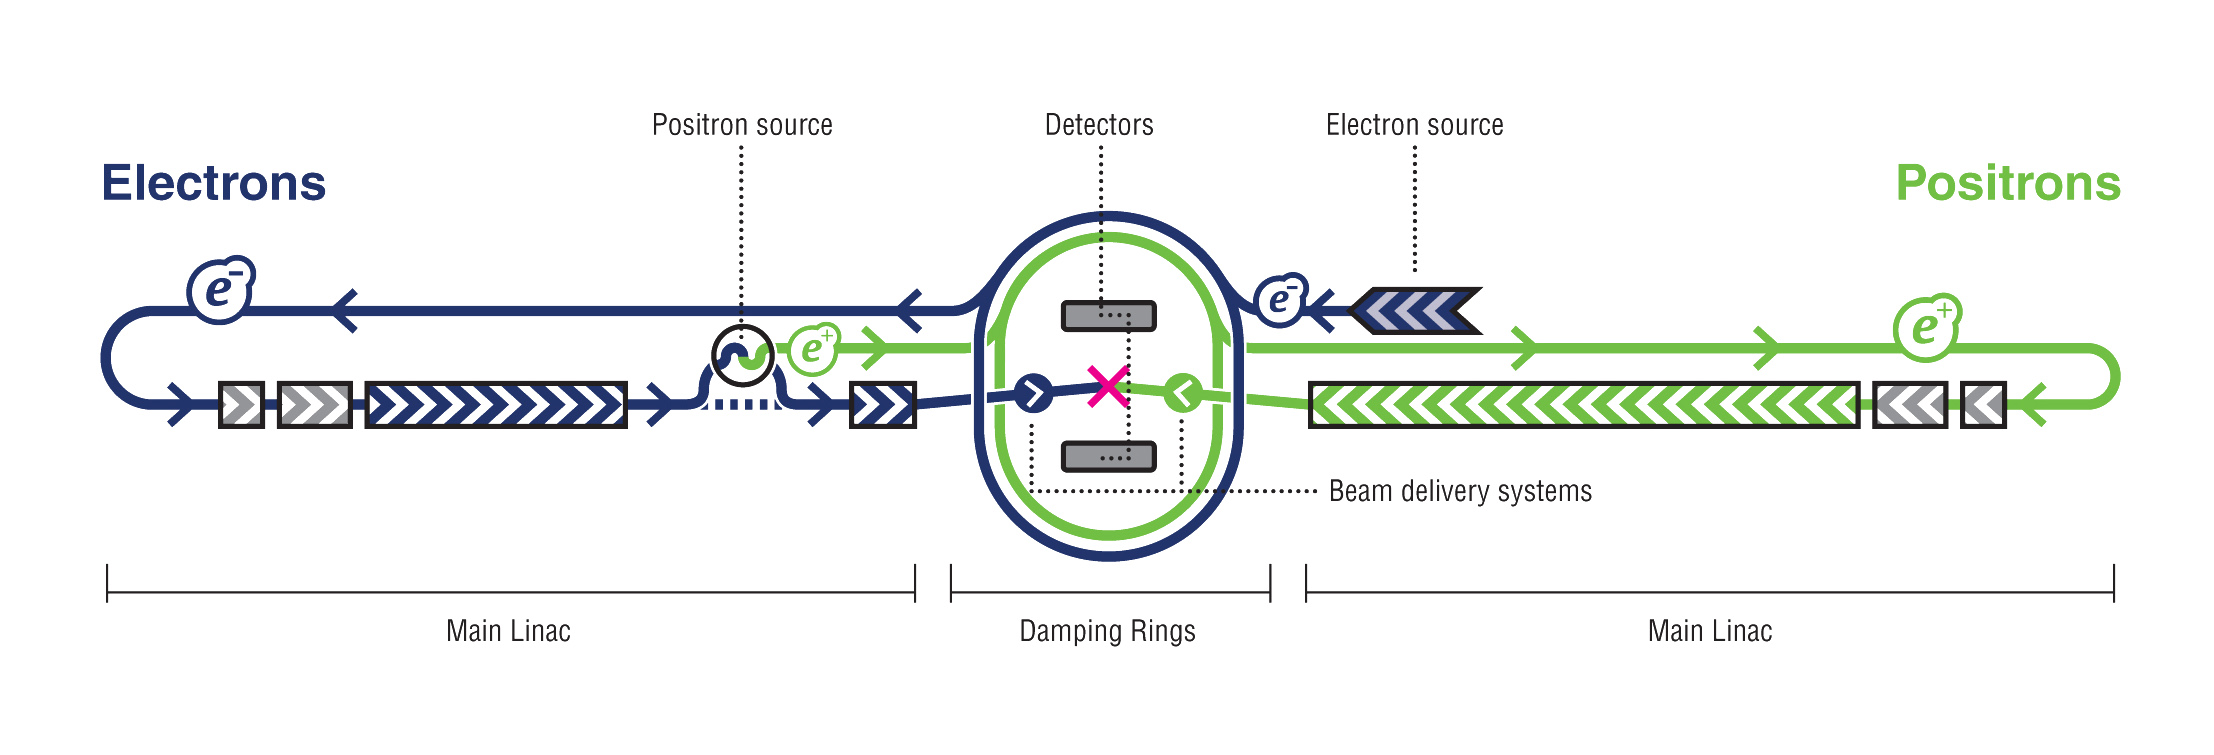
\includegraphics[width=0.95\textwidth]{graphics/ILC_scheme.jpg}
		\caption{\sl Vue sch\'ematique de l'ILC.}
		\label{fig:ILCSchemeF}
	}
\end{figure}

L’ILC devrait avoir deux d\'etecteurs, SiD et ILD, qui vont fonctionner de mani`ere alternative pour assurer la v\'erification des r\'esultats.
Cette th\'es\`e est concentr\'e sur l'experiance ILD. 

Le International Large Detector (ILD) est un concept pour un détecteur multi-usages de haute précision, conçu pour atteindre les objectifs de physique de l'ILC~\cite{Behnke:2013lya}.
%La vue schématique de l'ILD est présentée dans la Figure~\ref {fig:ILCSchemeF}.
Comme montr\'e dans la vue schématique, Fig.~\ref {fig:ILCSchemeF}, l’ILD est compos\'e de plusieurs sous-d\'etecteurs, plac\'es les uns autour des autres:
\begin{itemize}
	\item un d\'etecteur de vertex \'a pixel multicouche (VTX);
	\item une ”Time Projection Chamber” (TPC) comme d\'etecteur des traces centrale;
	\item un calorim\`etre \'electromagn\'etique hautement granulaire (ECAL);
	\item un calorim\`etre hadronique hautement granulaire (HCAL);
	\item une bobine supraconductrice, qui cr\'ee un champ B axial de 3.5~Tesla.
	\item un d\'etecteur de muons et des queues des cascades hadroniques (TCMT).
\end{itemize}

\begin{figure}
	\centering
	\begin{subfigure}{0.5\textwidth}
		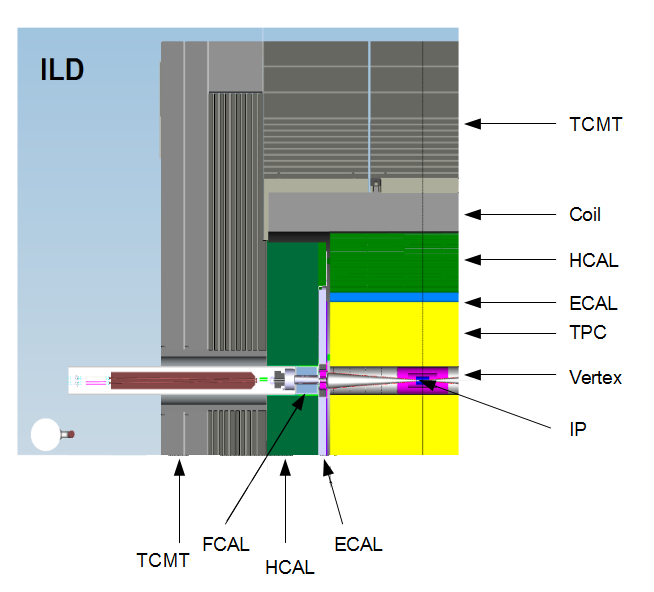
\includegraphics[width=0.95\textwidth]{graphics/ILD.png}
		
	\end{subfigure}% 
	\begin{subfigure}{0.5\textwidth}
		\centering
		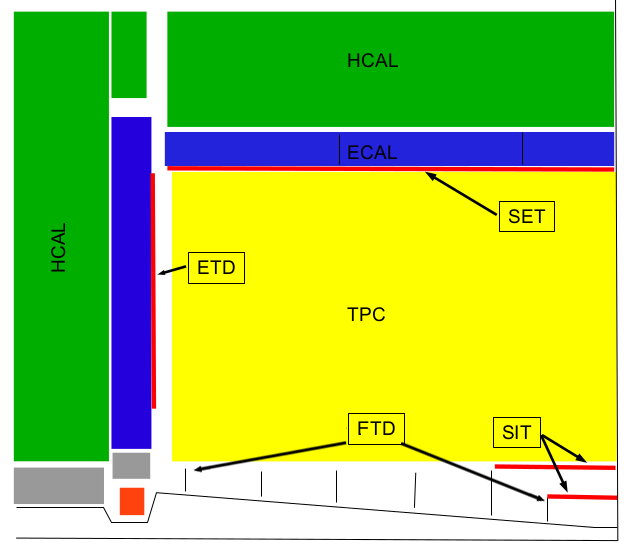
\includegraphics[width=0.9\textwidth]{graphics/ILDtracking.png}
		
	\end{subfigure}
	\caption{\sl Gauche: Vue sch\'ematique de l'ILD. Droite: Zoom sur les détecteurs internes.}
	\label{fig:ILDSchemeF}
\end{figure}
%-----------------------------------------------------------------------------
%-----------------------------------------------------------------------------
%-----------------------------------------------------------------------------
\newpage
\subsection*{Calorim\`etre \'electromagn\'etique silicium-tungst\`ene hautement granulaire}

Un calorim\`etre \'electromagn\'etique de silicium tungst\`ene (SiW-ECAL) est le
choix standard pour des concepts de d\'etecteur ILD.

La collaboration de CALICE (CAlorimetry for the LInear Collider Experiments) a construit et testé un prototype SiW-ECAL, la vue schématique du prototype est présentée dans la Figure~\ref {fig:ECAL-schemeF}.

Le tungst\'ene a l’avantage d’avoir une grande longueur d’interaction ($\lambda_I = 96$\,mm), compar\'ee \`a son $X_0$, ce
qui conduit \`a une bonne s\'eparation entre les photons et les hadrons dans un ECAL. 
Du silicium avec une taille de pixel de $1\times1$\,cm$^2$ est utilis\'e comme mat\'eriau actif dans le prototype. 
\begin{figure}
	\centering
	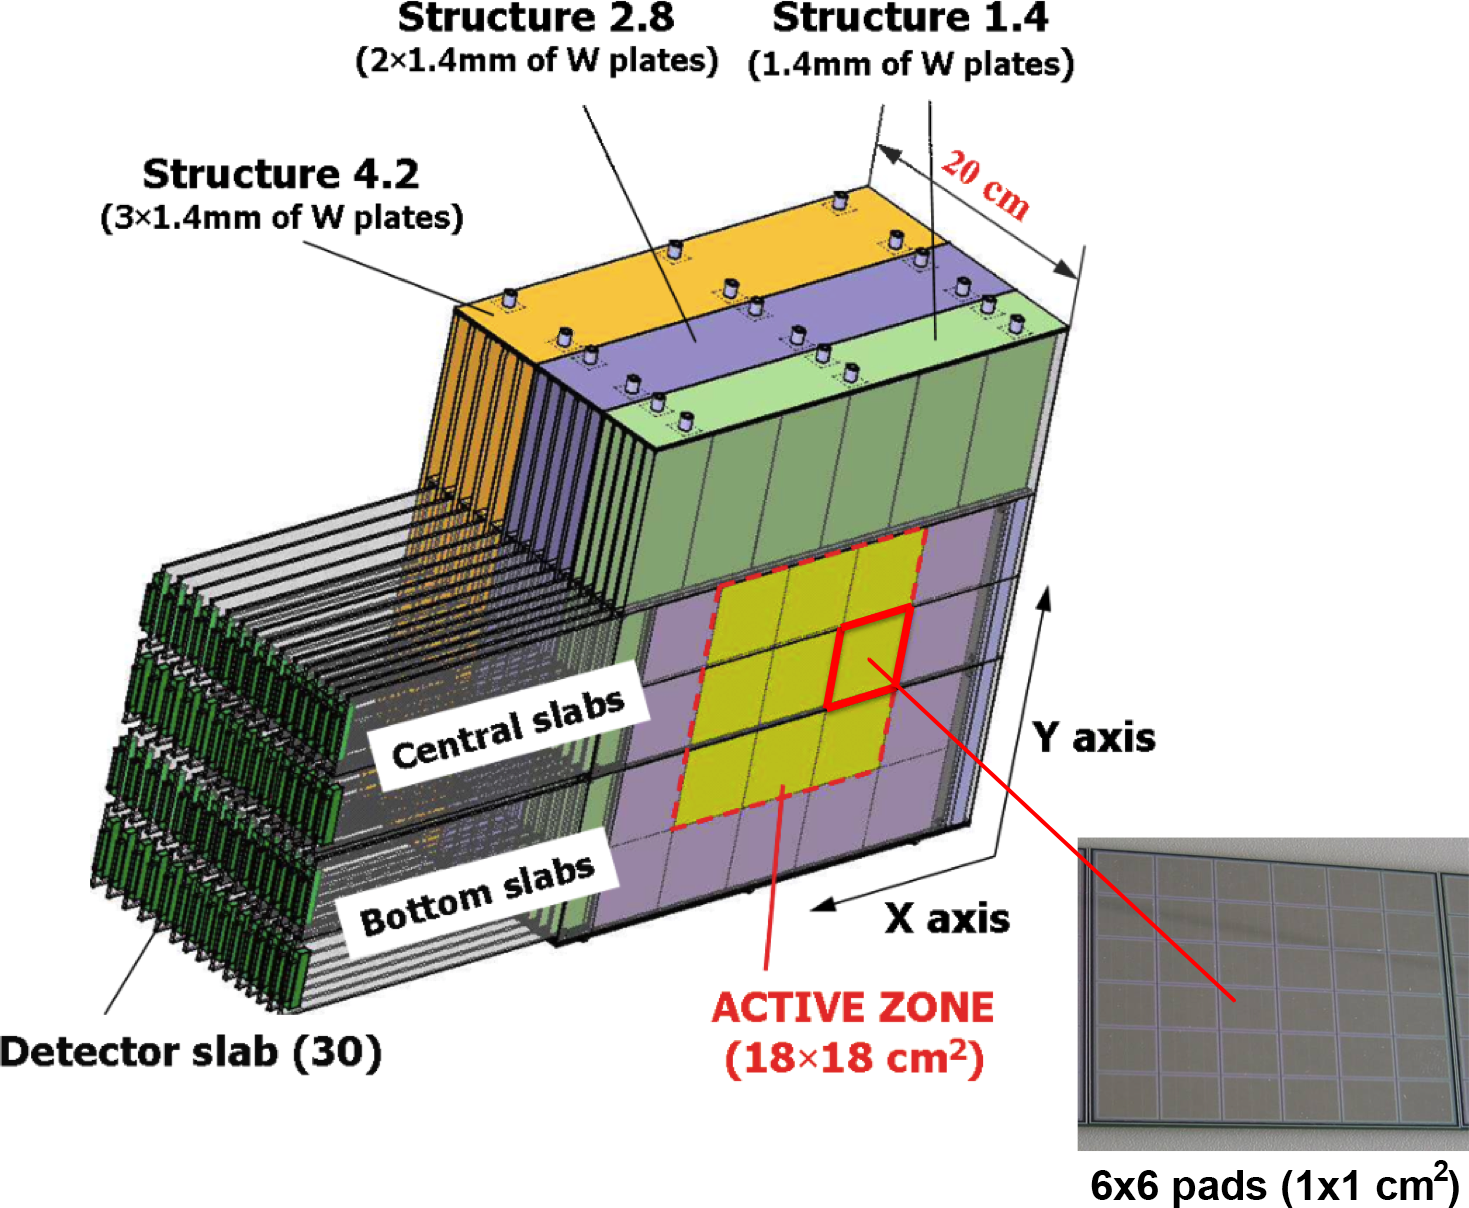
\includegraphics[width=0.55\textwidth]{ECAL/graphics/ecal-new.png}
	\caption{\label{fig:ECAL-schemeF} \sl  Vue sch\'ematique de \ecal.}
\end{figure}

%-----------------------------------------------------------------------------
%-----------------------------------------------------------------------------
%-----------------------------------------------------------------------------
\newpage
\subsection*{L'algorithme de reconstruction des traces}
L'objectif principal de l'algorithme de tracking developp\'ee est la détection de traces dispersées vers l'avant à partir de l'interaction entre les pions primaires et le matériau absorbant en l'absence d'un champ magnétique.

L'algorithme d\'esign\'e comporte le sch\'ema d'ex\'ecution suivant:
\begin{itemize}
	\item La région d'interaction est identifiée en utilisant un critère topologique et séparée pour une analyse plus approfondie, voir Fig.~\ref{fig:testF};
	\item Les dépositions d'énergie restantes sont utilisées pour un algorithme de clusterization, voir Fig.~\ref{fig:democlusterF};
	\item Les clusters obtenues sont classées pour sélectionner des clusters similaires à des traces provenant du bruit résiduel;
	\item Après la classification, clusters différents d'une seule particule secondaire  sont fusionnés en une seule trace.
	
\end{itemize}
\begin{figure}
	\centering
	\begin{subfigure}{0.5\textwidth}
		\centering
		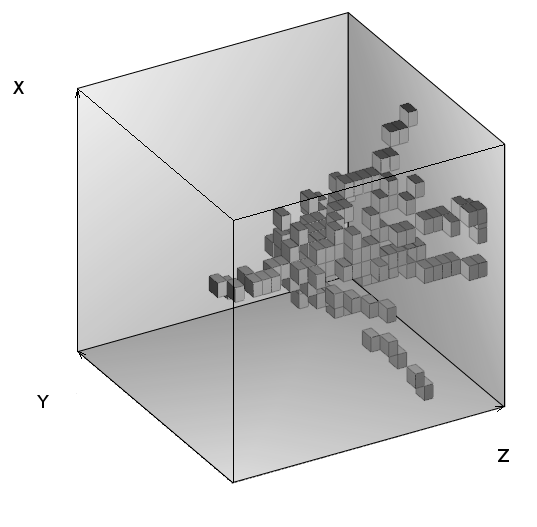
\includegraphics[width=.90\linewidth]{ECAL/graphics/before.png}
		\caption{\label{fig:beforeF} \sl avec région d'interaction.}
	\end{subfigure}% 
	\begin{subfigure}{0.5\textwidth}
		\centering
		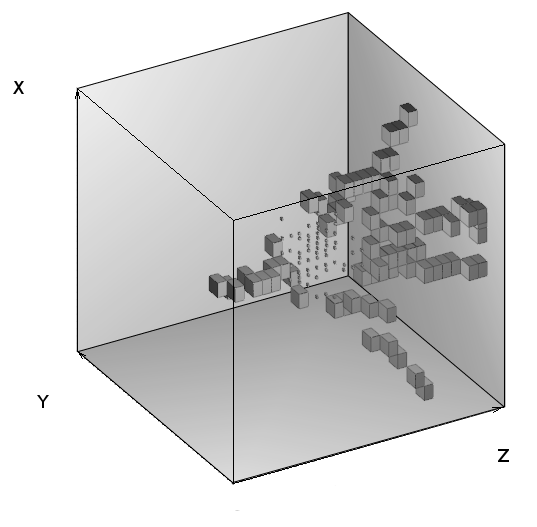
\includegraphics[width=.90\linewidth]{ECAL/graphics/after2.png}
		\caption{\label{fig:afterF} \sl sans région d'interaction.}
	\end{subfigure}
	\caption{ \sl Visualisation d'événement de l'interaction pion primaire avec 10\,GeV d'energie enregistré au FNAL 2008 avant \textit{(a)} et apr\'es suppression de la région d'interaction\textit{(b)}. }
	%Event 16-17 in Data10.root
	\label{fig:testF}
\end{figure}


\begin{figure}
	\centering
	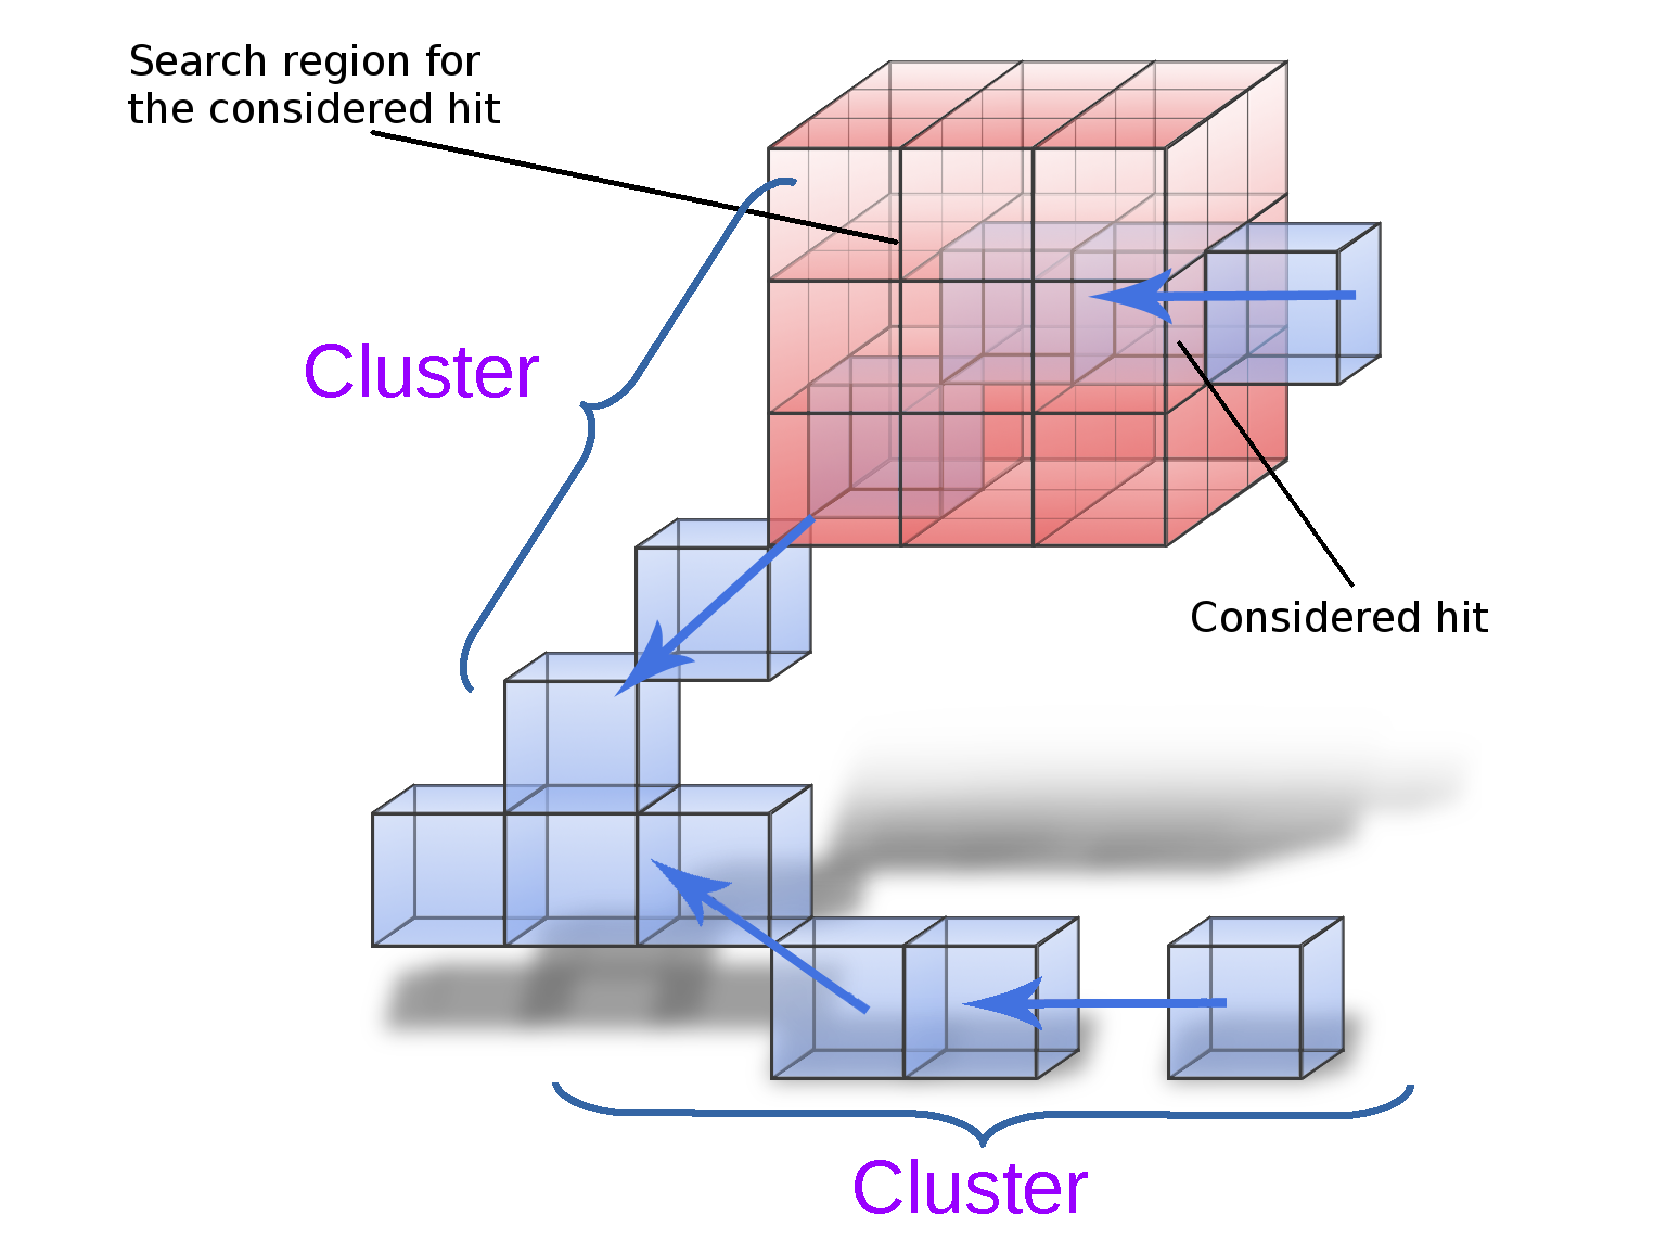
\includegraphics[width=0.55\textwidth]{ECAL/graphics/demo-v3.pdf}
	\caption{\label{fig:democlusterF} \sl Illustration de l'étape de clusterization. Les pixels actives sont représentés par des cubes bleus, et la zone de recherche pour les impacts adjacents est indiquée par des cubes rouges. Les flèches bleues indiquent la direction du flux de clusterization.}
\end{figure}

%-----------------------------------------------------------------------------
%-----------------------------------------------------------------------------
%-----------------------------------------------------------------------------
\newpage
\subsection*{Comparaison des simulations avec les données réelles}


La figure \ref{fig:irexampleF} montre les comparaisons des distributions d'énergie de la région d'interaction sur le dépôt d'énergie total $f_ {IR}$ entre les données et les trois listes de physique de {\sc Geant4}.
Le premier bac de ces histogrammes correspond à la fraction d'événements pour laquelle aucune region d'interaction n'est trouvée par l'algorithme.


\begin{figure}
	\centering
	\begin{subfigure}{0.5\textwidth}
		\centering
		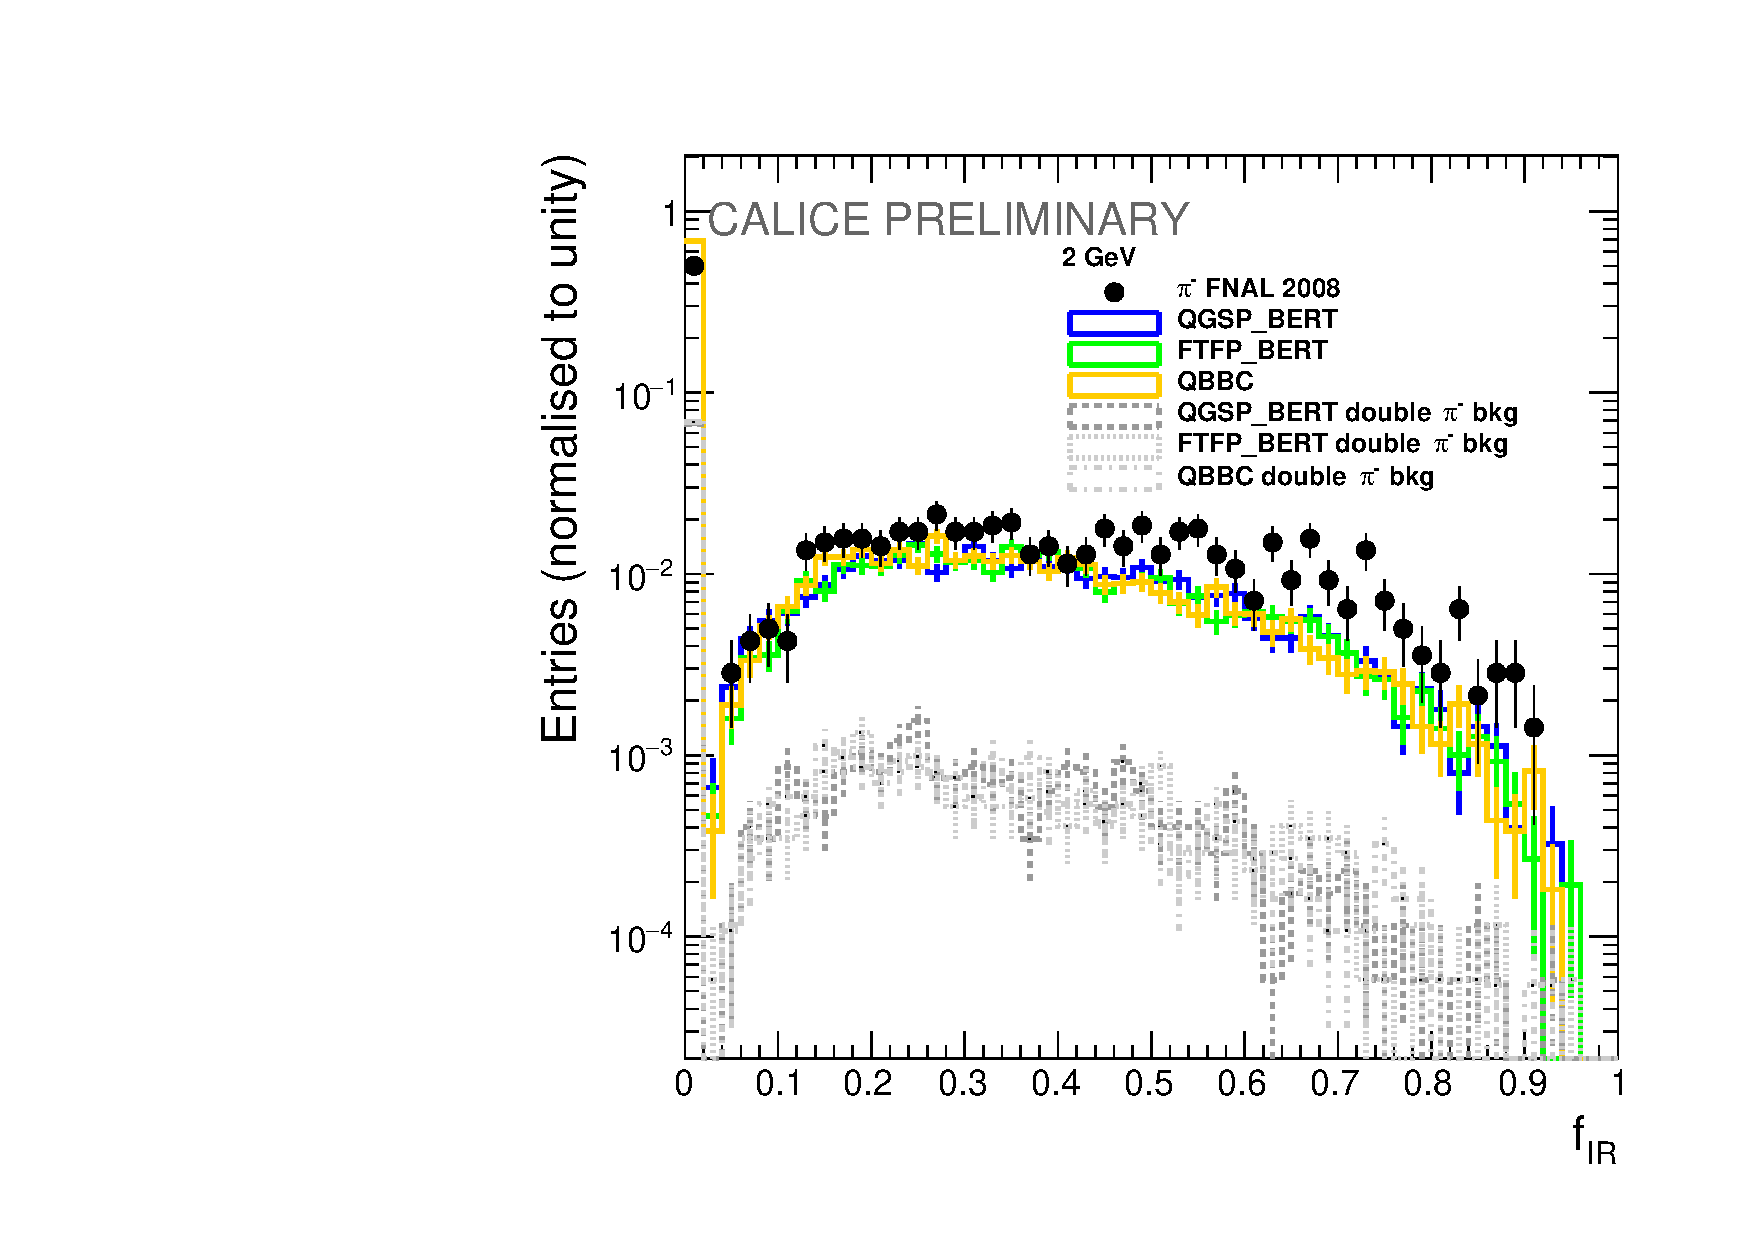
\includegraphics[width=.90\linewidth]{ECAL/plots/e-ir-2.pdf}
		\caption{\label{fig:efr2F} }
	\end{subfigure}% 
	\begin{subfigure}{0.5\textwidth}
		\centering
		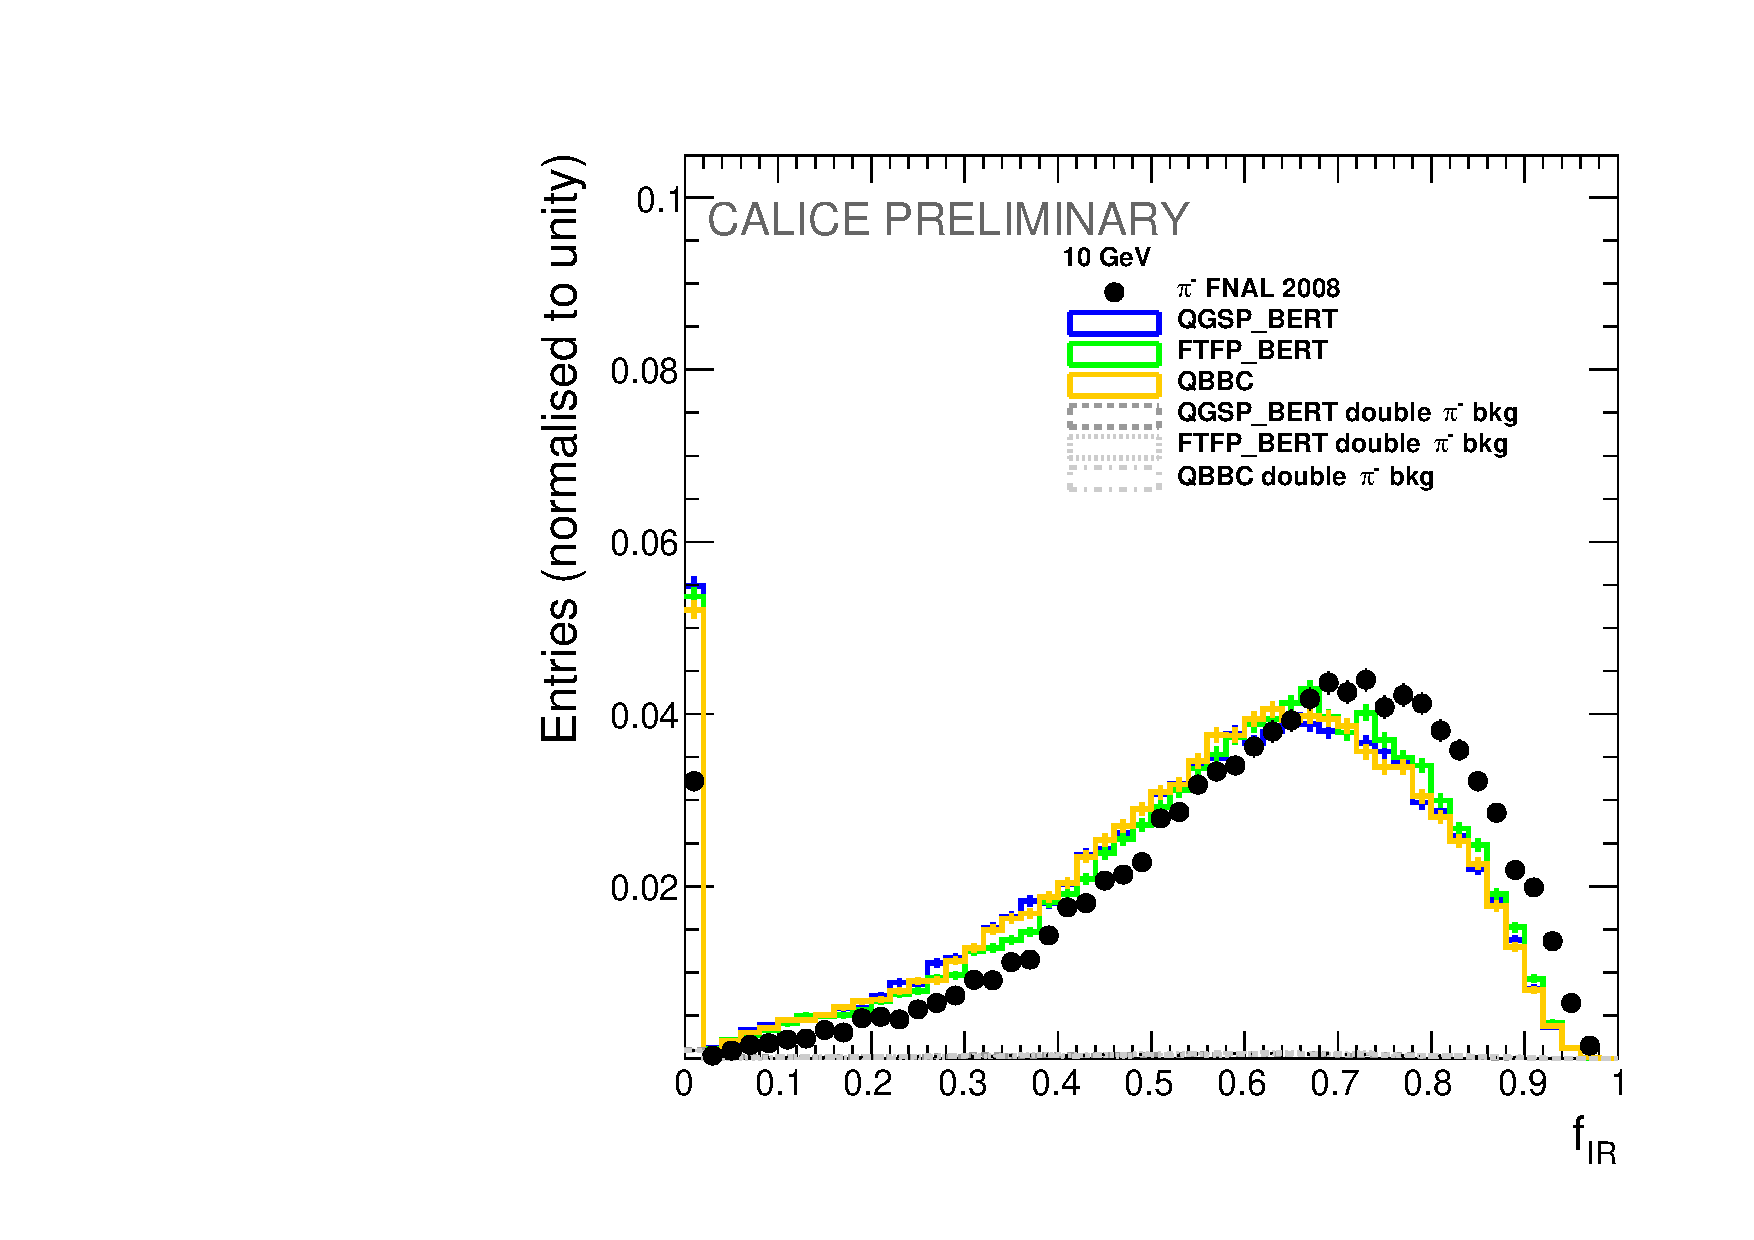
\includegraphics[width=.90\linewidth]{ECAL/plots/e-ir-10.pdf}
		\caption{\label{fig:efr10F} }
	\end{subfigure}
	\caption{\label{fig:irexampleF} \sl% {\bf Fig.~\ref{fig:efr2}: Remind me how the linear plot looks like} 
		Comparaison de $f_{IR}$ entre les données et les simulations pour trois {\sc Geant}4  listes physiques de l'\'energies 2 (a) et 10 (b) GeV de particule primordiale.}
\end{figure}

Dans la figure \ref{fig:irgraphF}, la valeur moyenne de $f_ {IR}$ est représentée en fonction de l'énergie du faisceau pour les énergies du faisceau de 2, 4, 6, 8 et 10 \, GeV.
Dans le cas de simulation, la valeur moyenne de $f_ {IR}$ est jusqu'à 20 \% inférieure à celle observée dans les données.

\begin{figure}
	\centering
	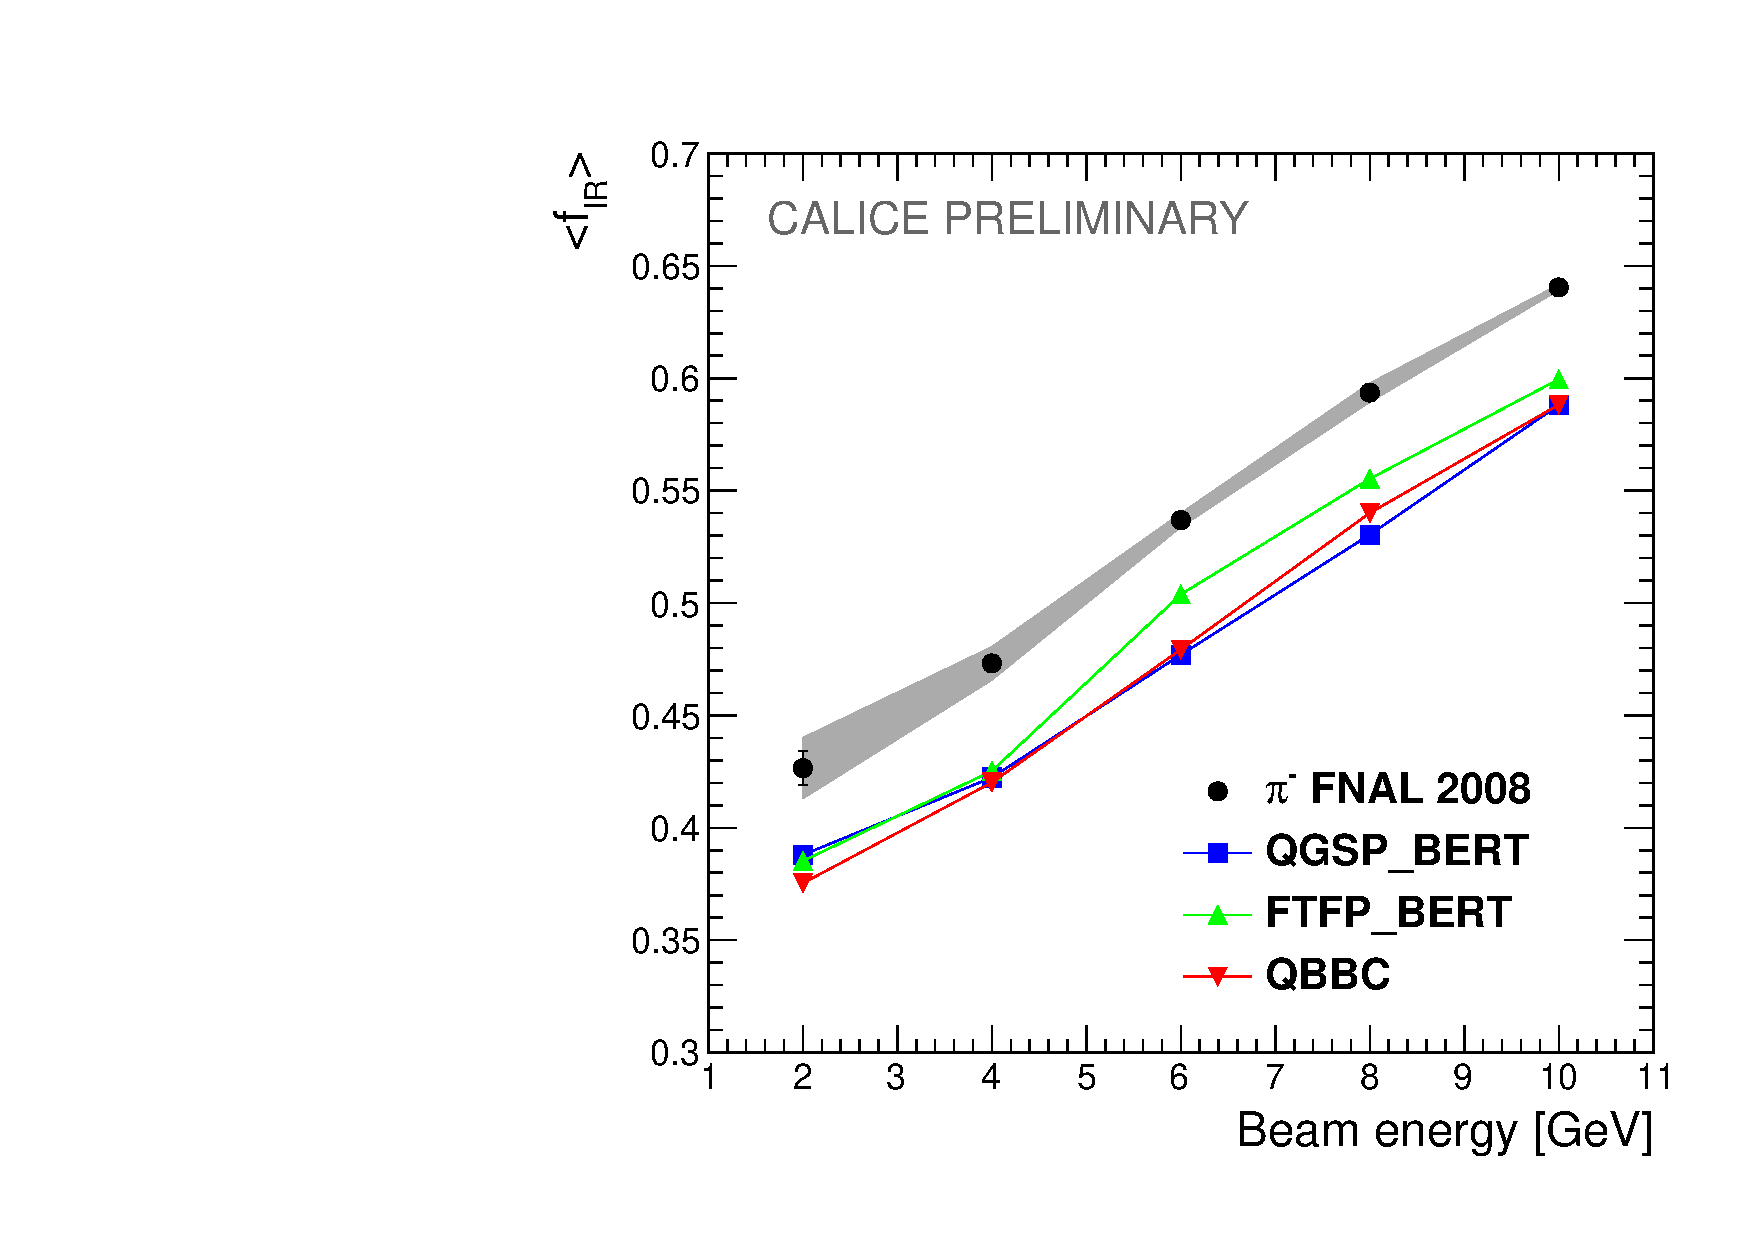
\includegraphics[width=0.5\textwidth]{ECAL/plots/e-ir-graph.pdf}
	\caption{\label{fig:irgraphF} \sl  Fraction moyenne du dépôt d'énergie dans la région d'interaction pour les données et les simulations  pour trois listes physiques \geant\ comme une fonction de l'énergie du faisceau (2 \, GeV à 10 \, GeV).}
\end{figure}

%\begin{figure}
%	\centering
%	\begin{subfigure}{0.5\textwidth}
%		\centering
%		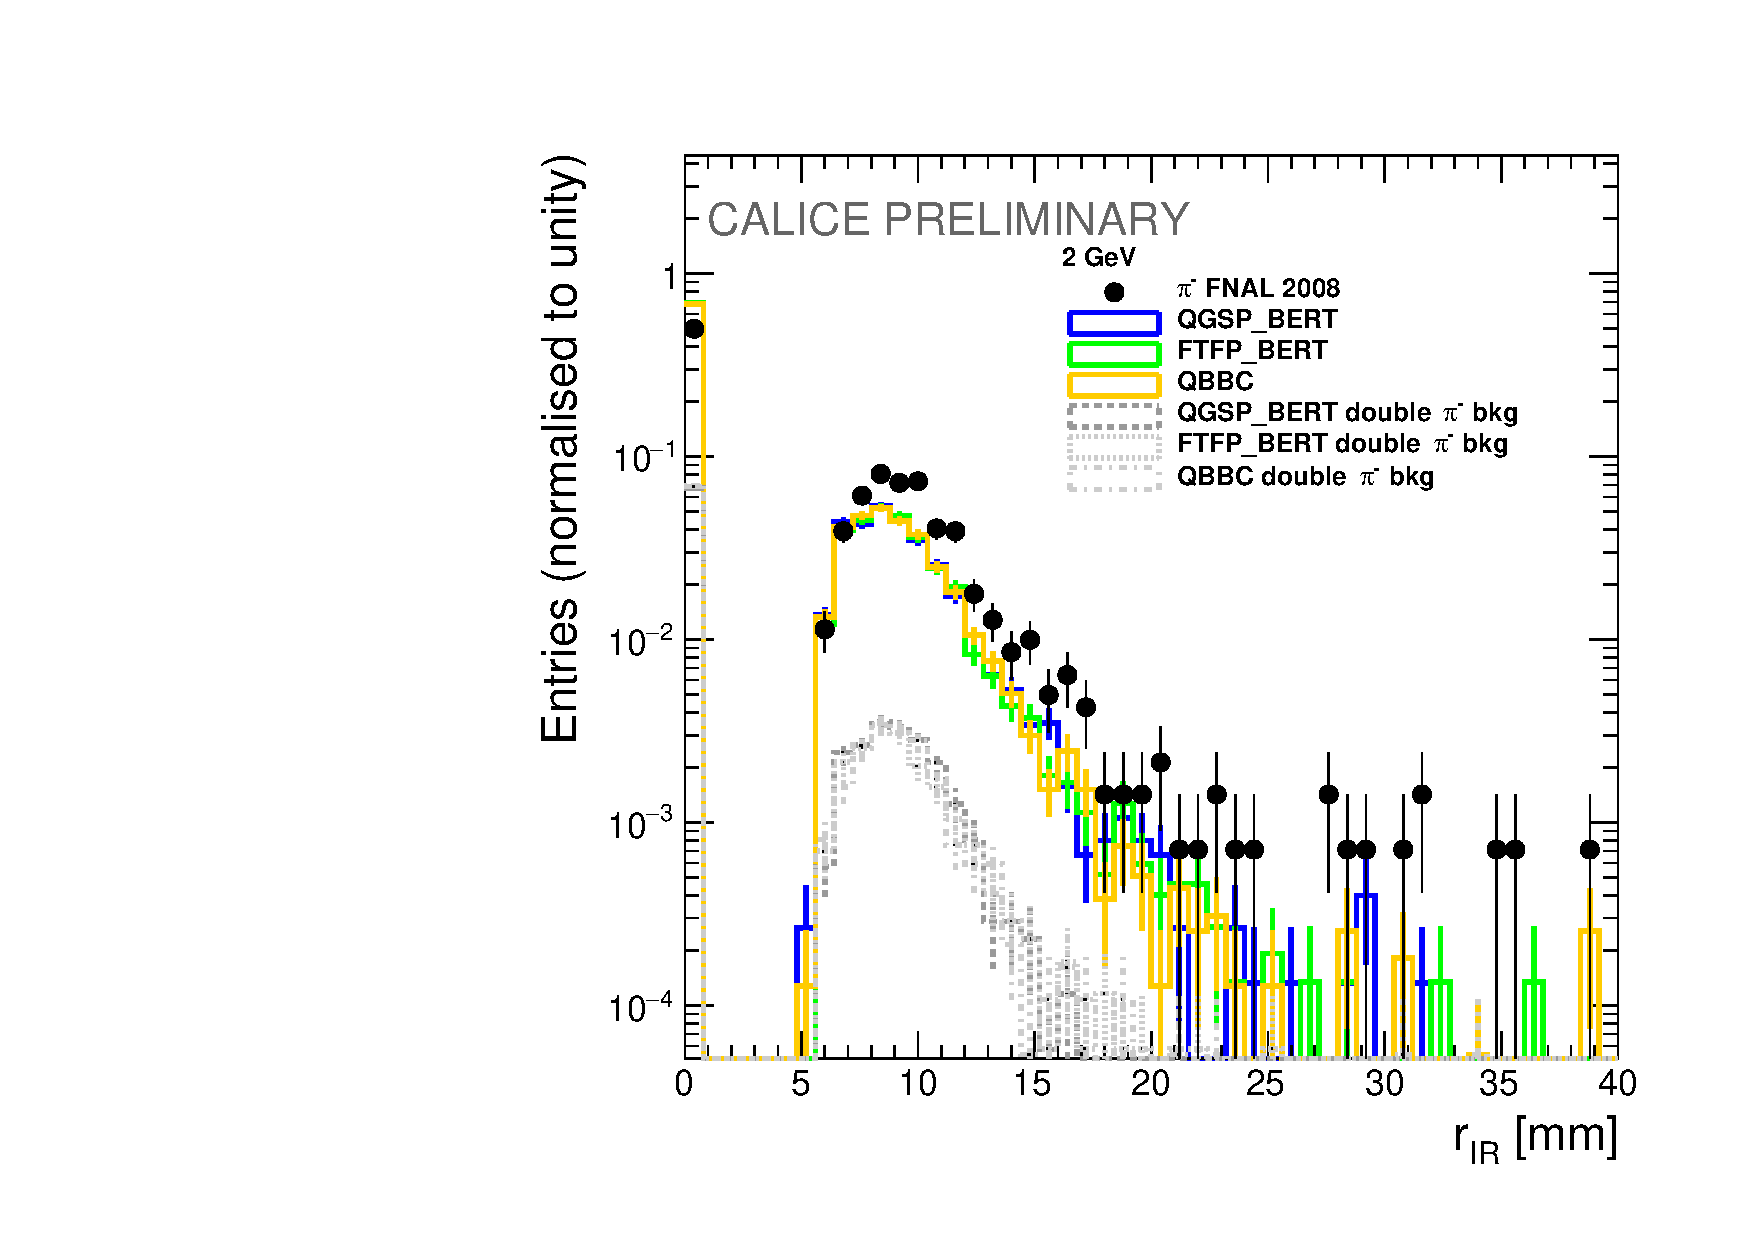
\includegraphics[width=.90\linewidth]{ECAL/plots/r-ir-2.pdf}
%		\caption{\label{fig:rir2F} }
%	\end{subfigure}% 
%	\begin{subfigure}{0.5\textwidth}
%		\centering
%		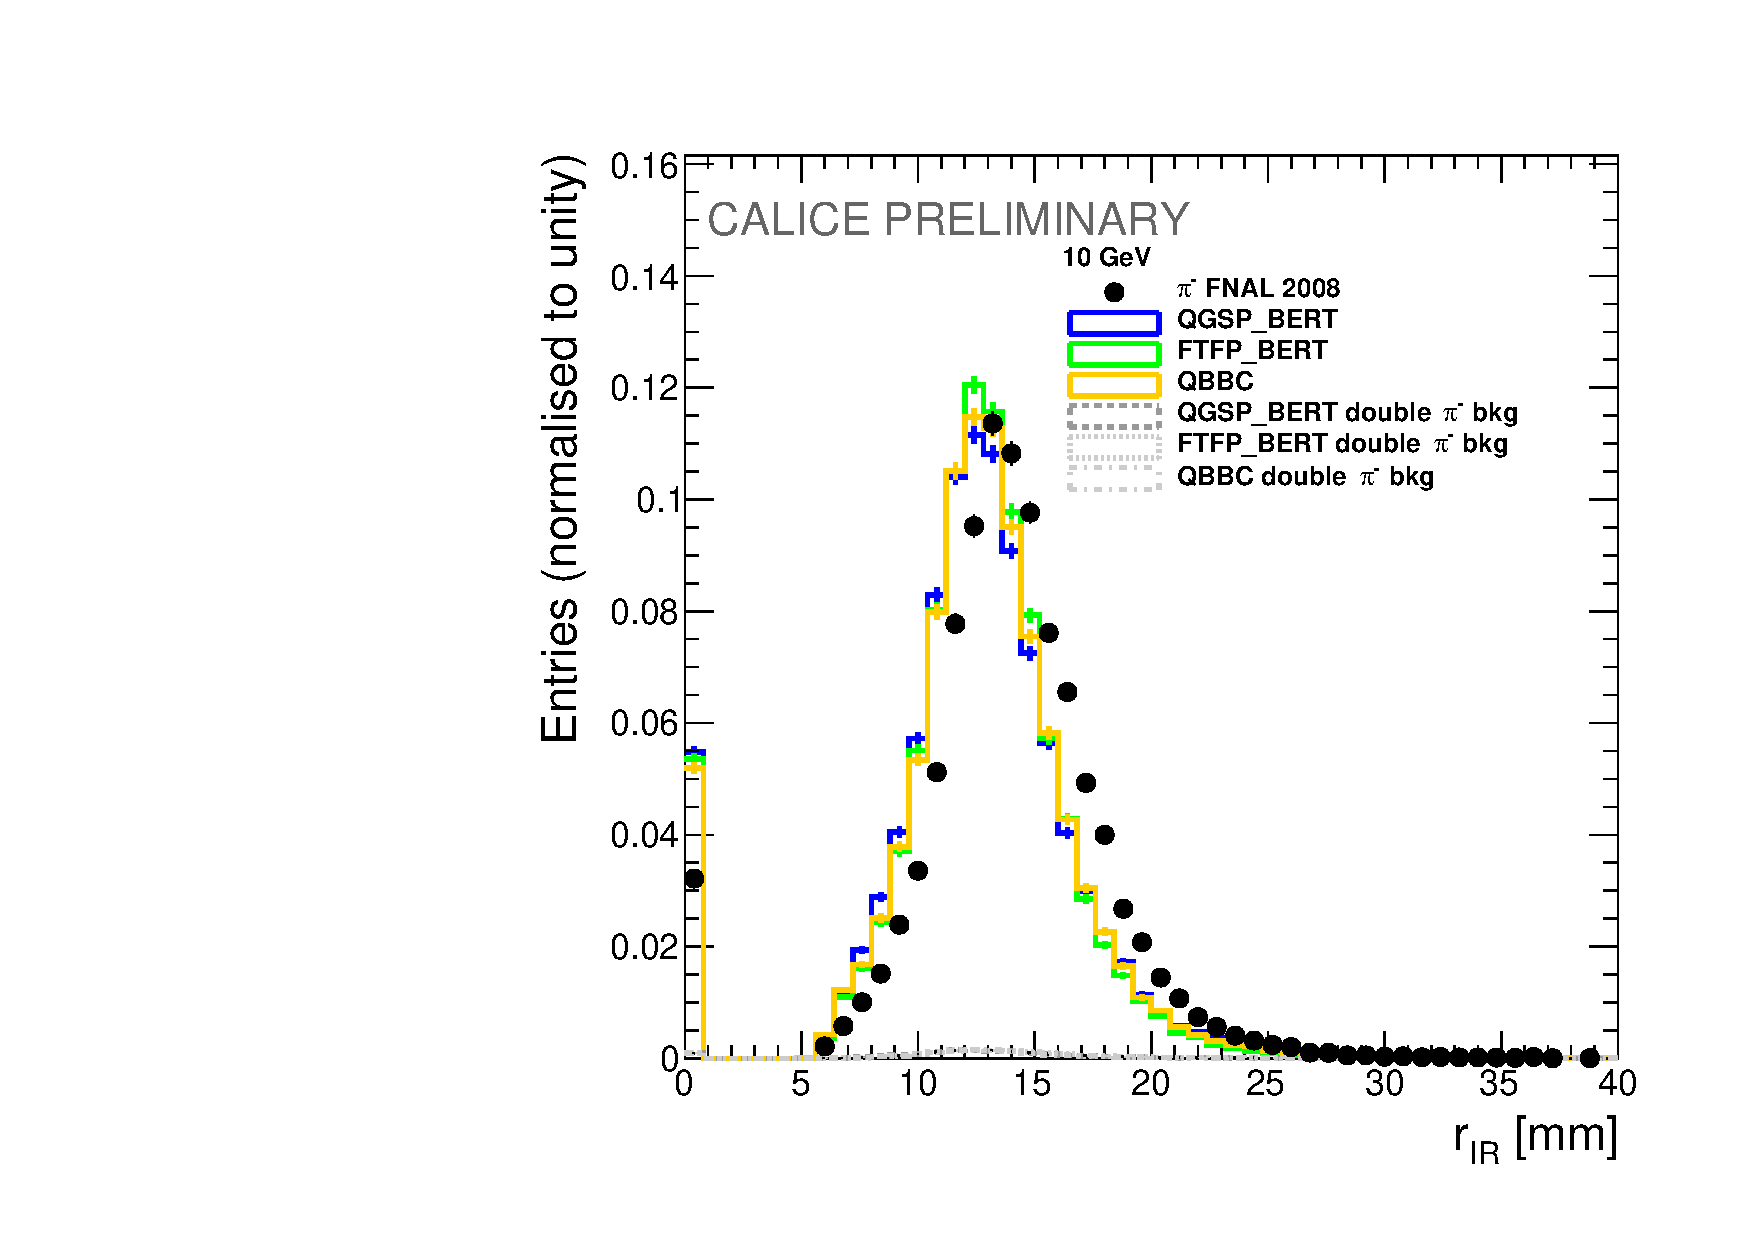
\includegraphics[width=.90\linewidth]{ECAL/plots/r-ir-10.pdf}
%	\end{subfigure}
%	\caption{\label{fig:rirexampleF} \sl %{\bf Same remark as for Fig.~\ref{fig:efr2} }
%		Comparaison de $r_{IR}$ entre les données et les simulations pour trois {\sc Geant}4  listes physiques de l'\'energies 2 (a) et 10 (b) GeV de particule primordiale.}
%\end{figure}

%\begin{figure}
%	\centering
%	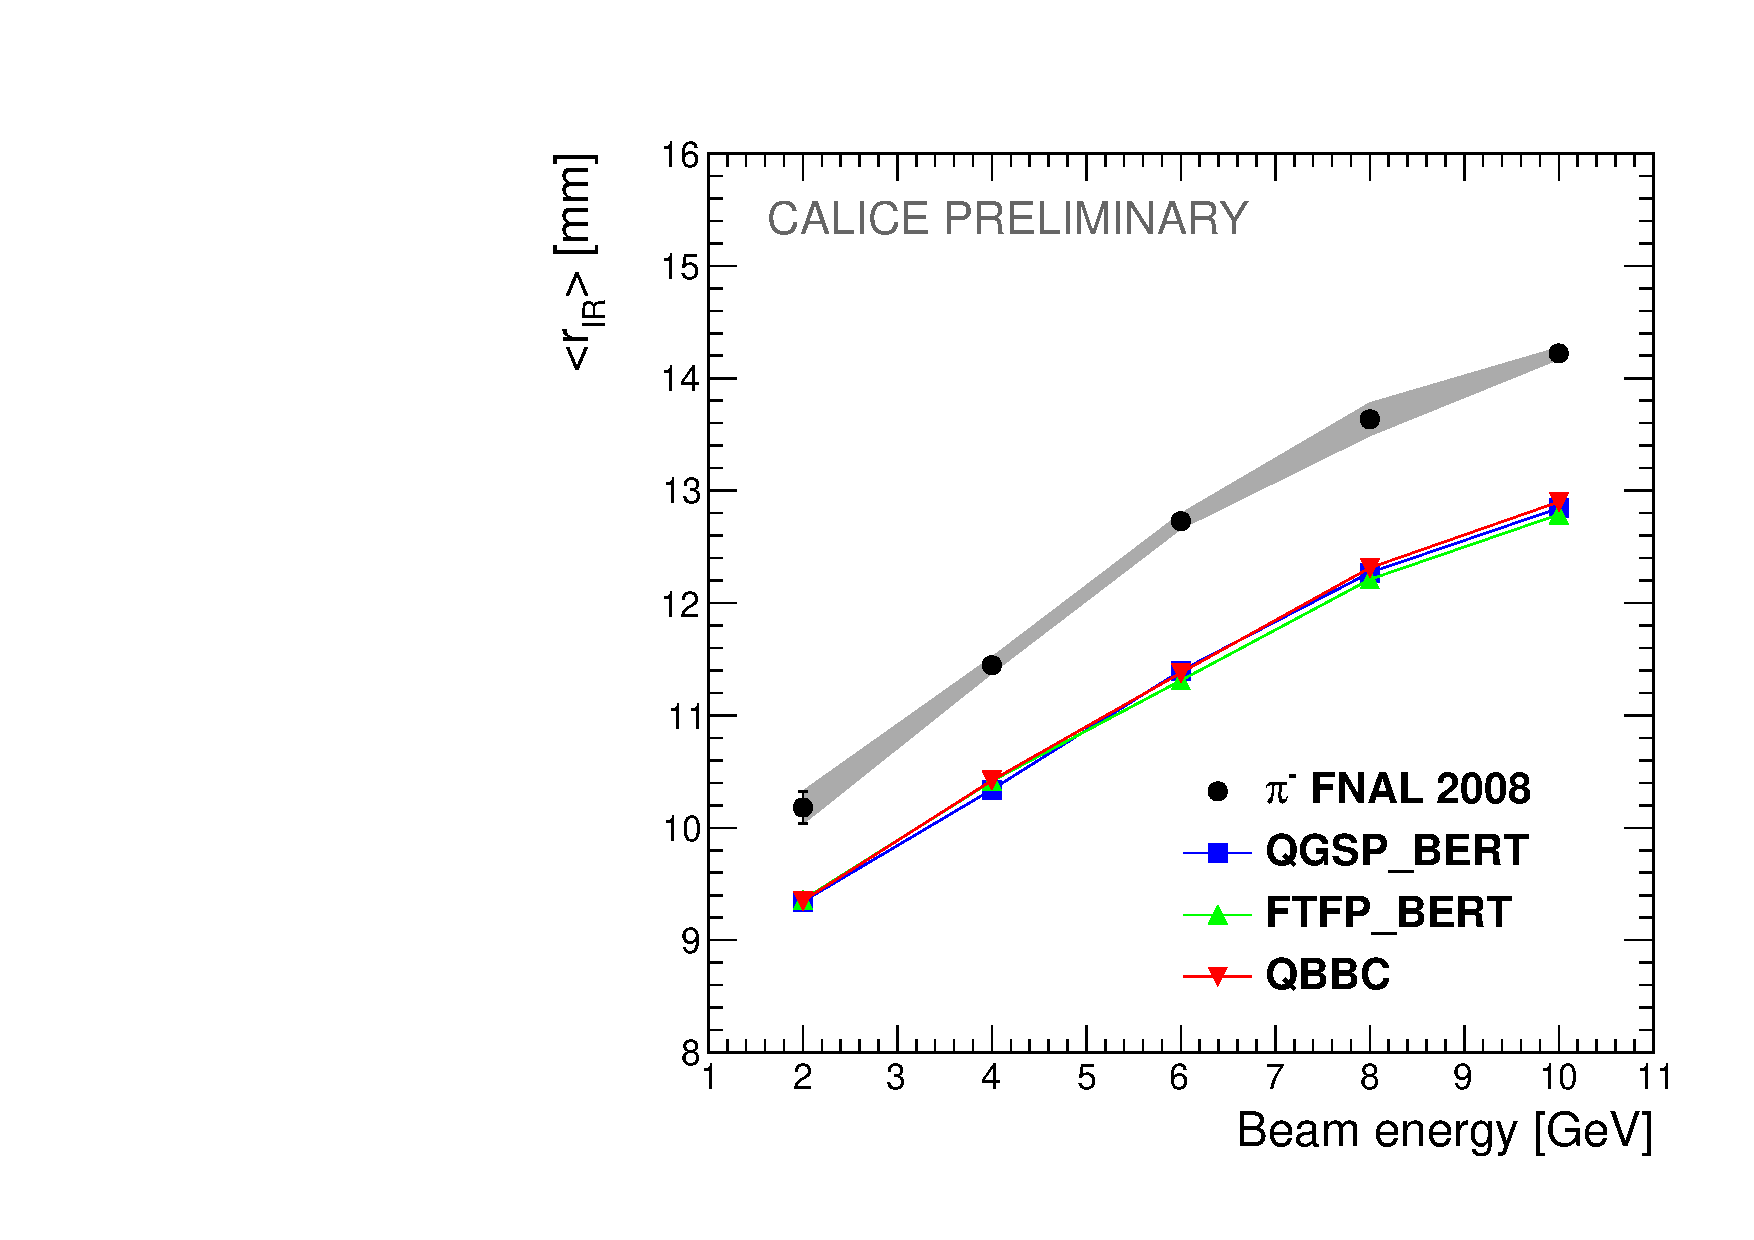
\includegraphics[width=0.5\textwidth]{ECAL/plots/r-ir-graph.pdf}
%	\caption{\label{fig:irrgraphF} \sl Radius lateral moyen de la région d'interaction pour les données et les simulations  pour trois listes physiques \geant\ comme une fonction de l'énergie du faisceau (2 \, GeV à 10 \, GeV).}
%\end{figure}

Un résultat central du l'algorithme de tracking developp\'ee est le nombre de traces secondaires ($N_ {tracks}$) et les observables en fonction de leurs propriétés.
Les distributions $N_ {tracks}$ sont présentées dans la Fig.~\ref{fig:NtrackF} pour les simulations de données et Monte Carlo sur la base des trois listes de physique {\sc Geant4} testées pour les énergies de 2 et 10\,GeV de l'entrant $\pi^-$-mesons.

Les trois listes de physique, présentées dans la Fig.~\ref{fig:fulltrackgraphF}, sous-estiment le nombre de traces secondaires de 7\% en moyenne inférieures à 10\,GeV et sont en accord avec les données à 10\,GeV.
\begin{figure}
	\centering
	\begin{subfigure}{0.5\textwidth}
		\centering
		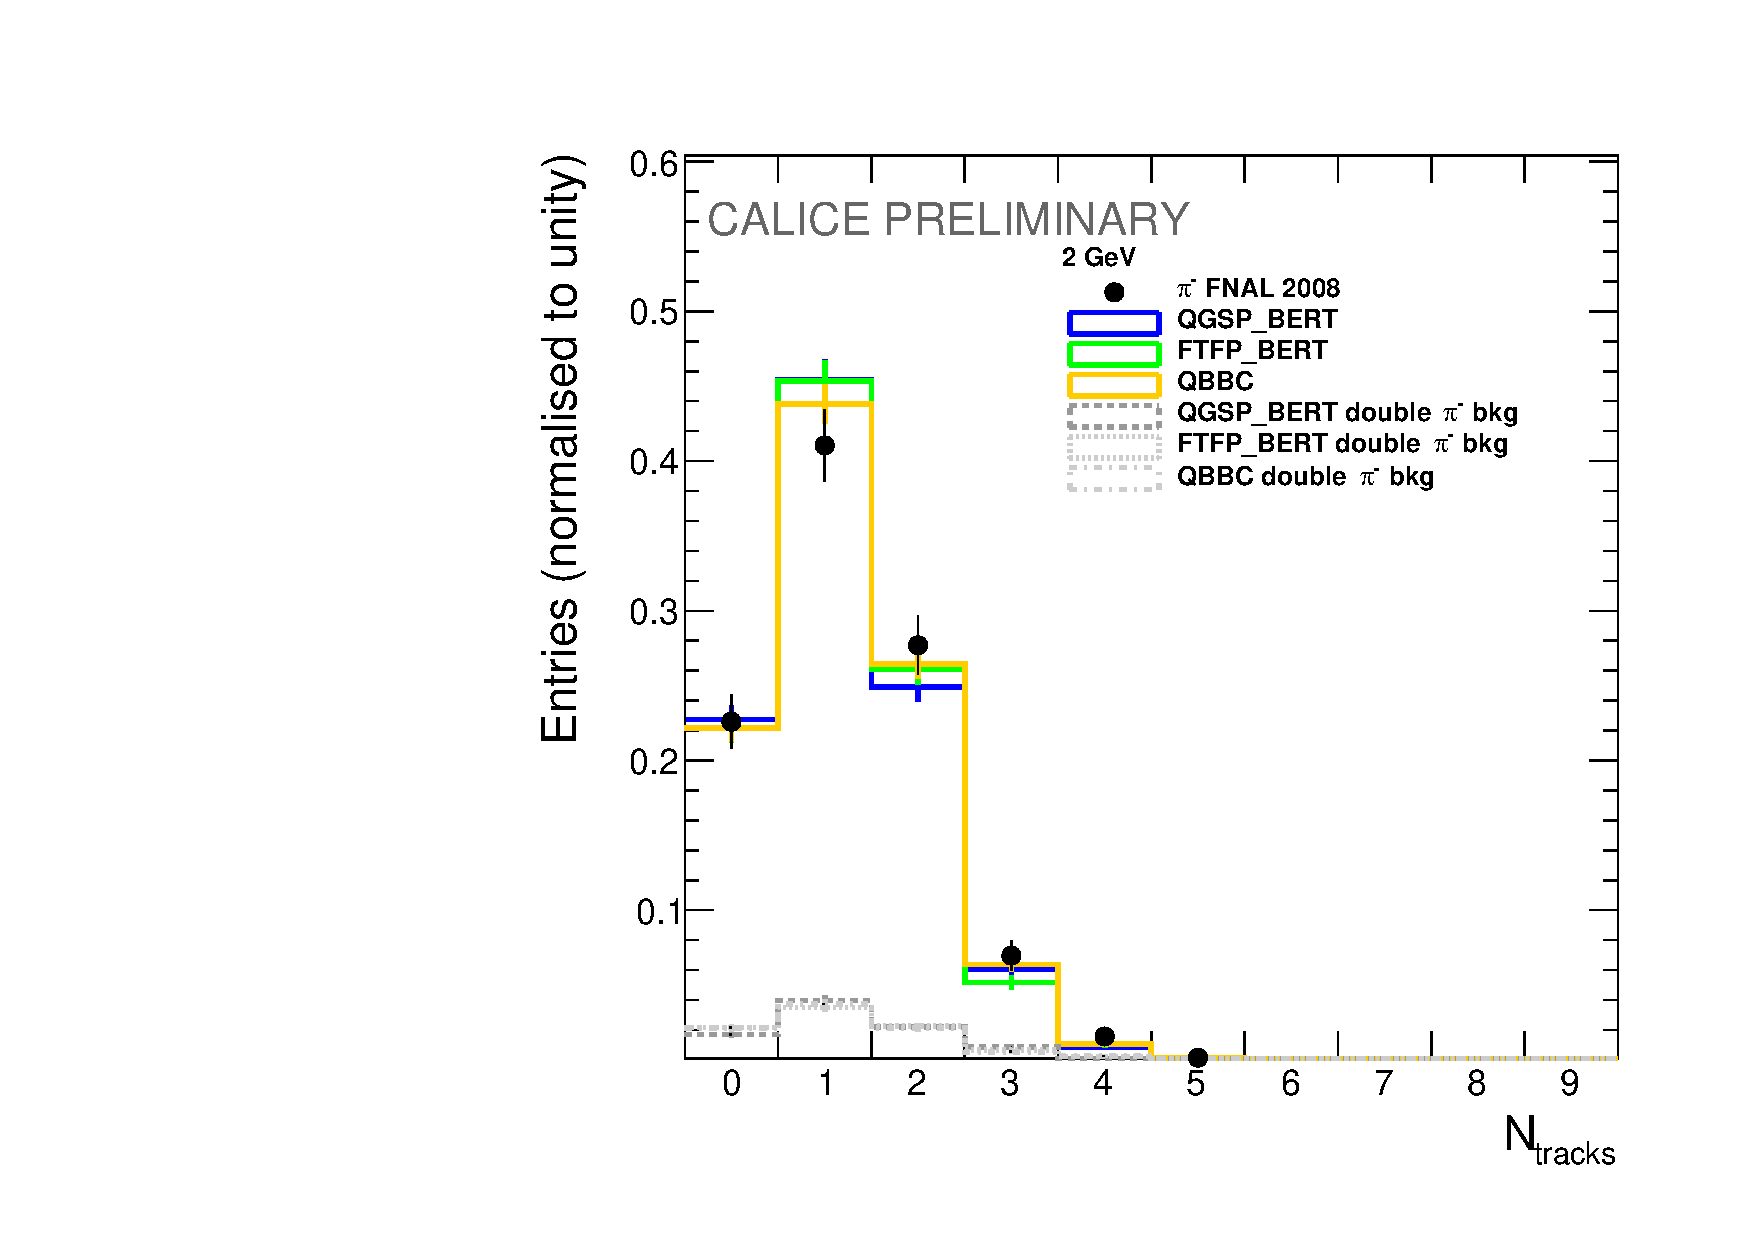
\includegraphics[width=.90\linewidth]{ECAL/plots/ntracks-2.pdf}
		\caption{\label{fig:tr2F} }
	\end{subfigure}% 
	\begin{subfigure}{0.5\textwidth}
		\centering
		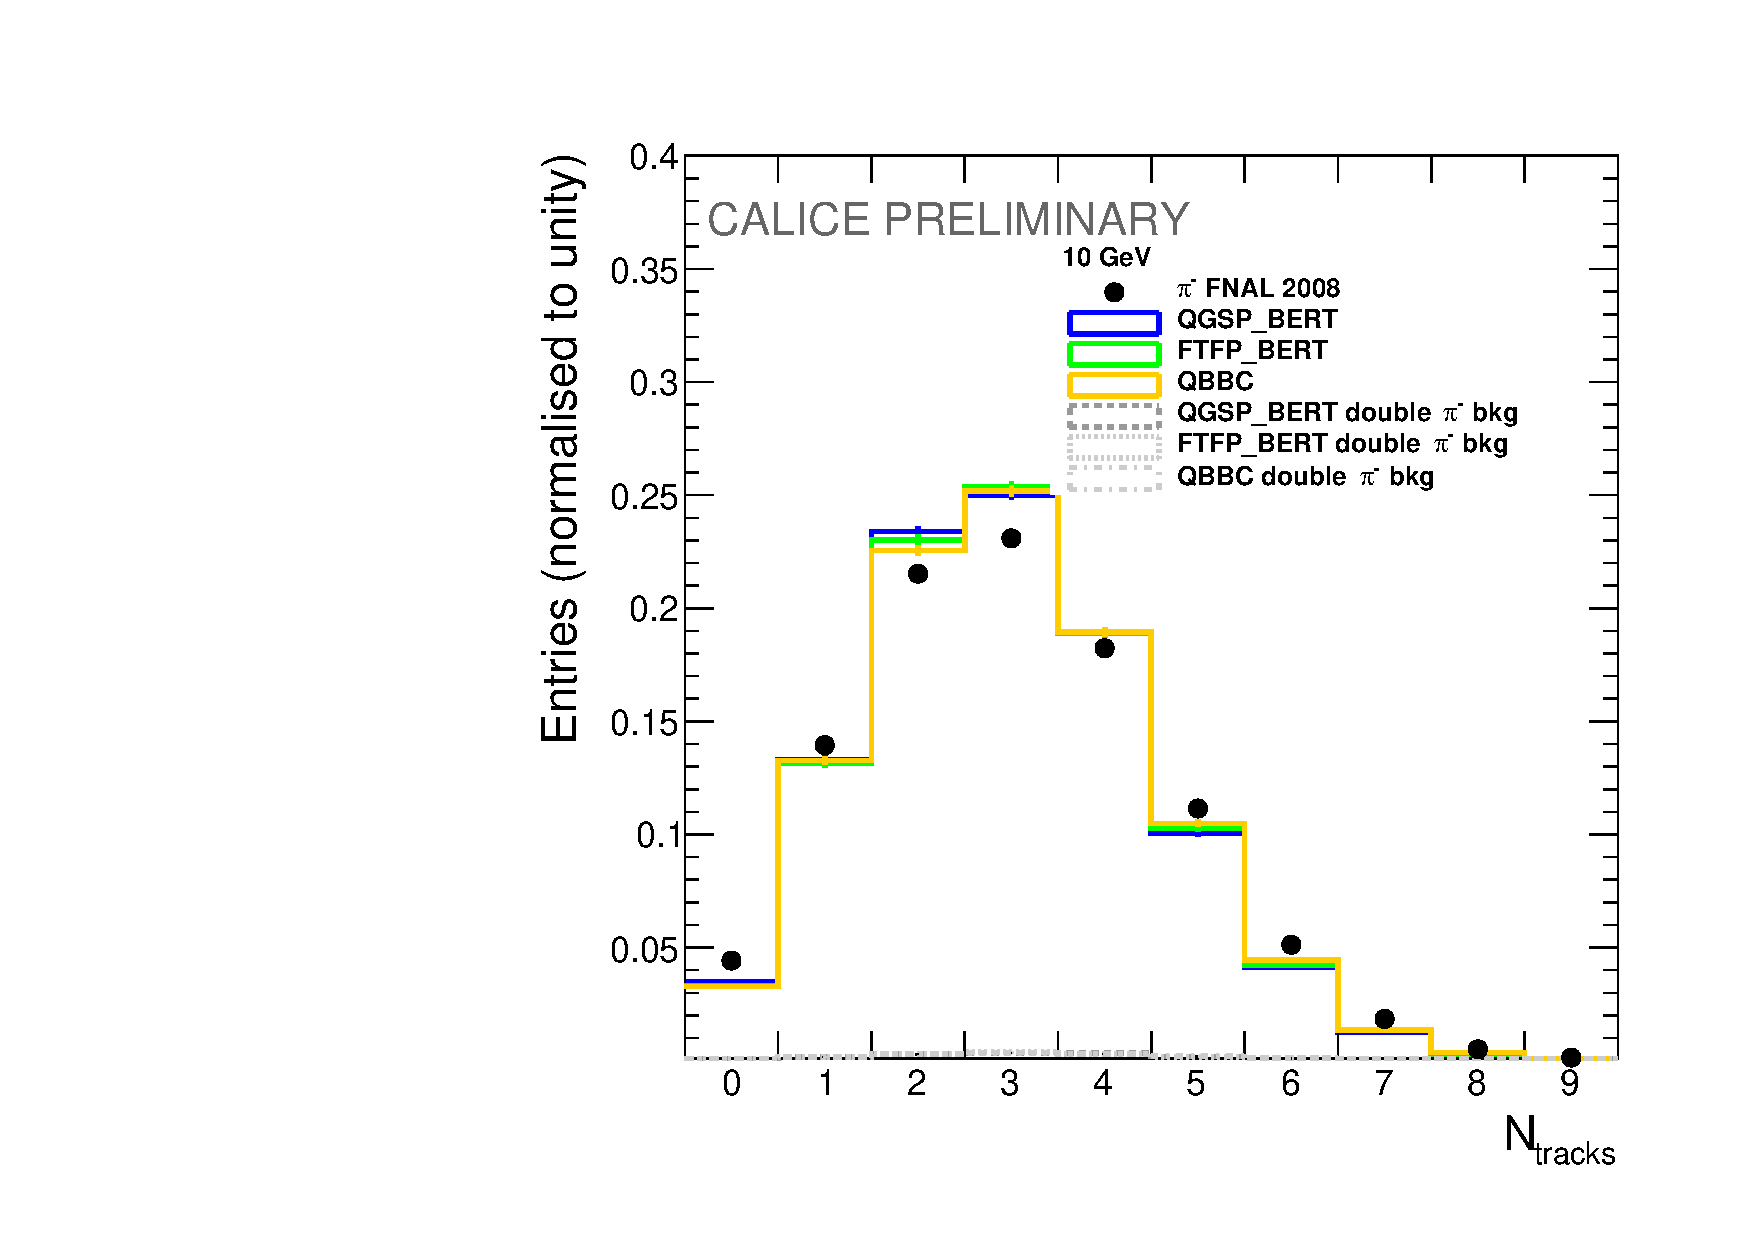
\includegraphics[width=.90\linewidth]{ECAL/plots/ntracks-10.pdf}
		\caption{\label{fig:tr10F} }
	\end{subfigure}
	\caption{\label{fig:NtrackF} \sl Comparaison de $N_{tracks}$ entre les données et les simulations pour trois {\sc Geant}4  listes physiques de l'\'energies 2 (a) et 10 (b) GeV de particule primordiale.}
\end{figure}

\begin{figure}
	\centering
	\begin{subfigure}{0.5\textwidth}
		\centering
		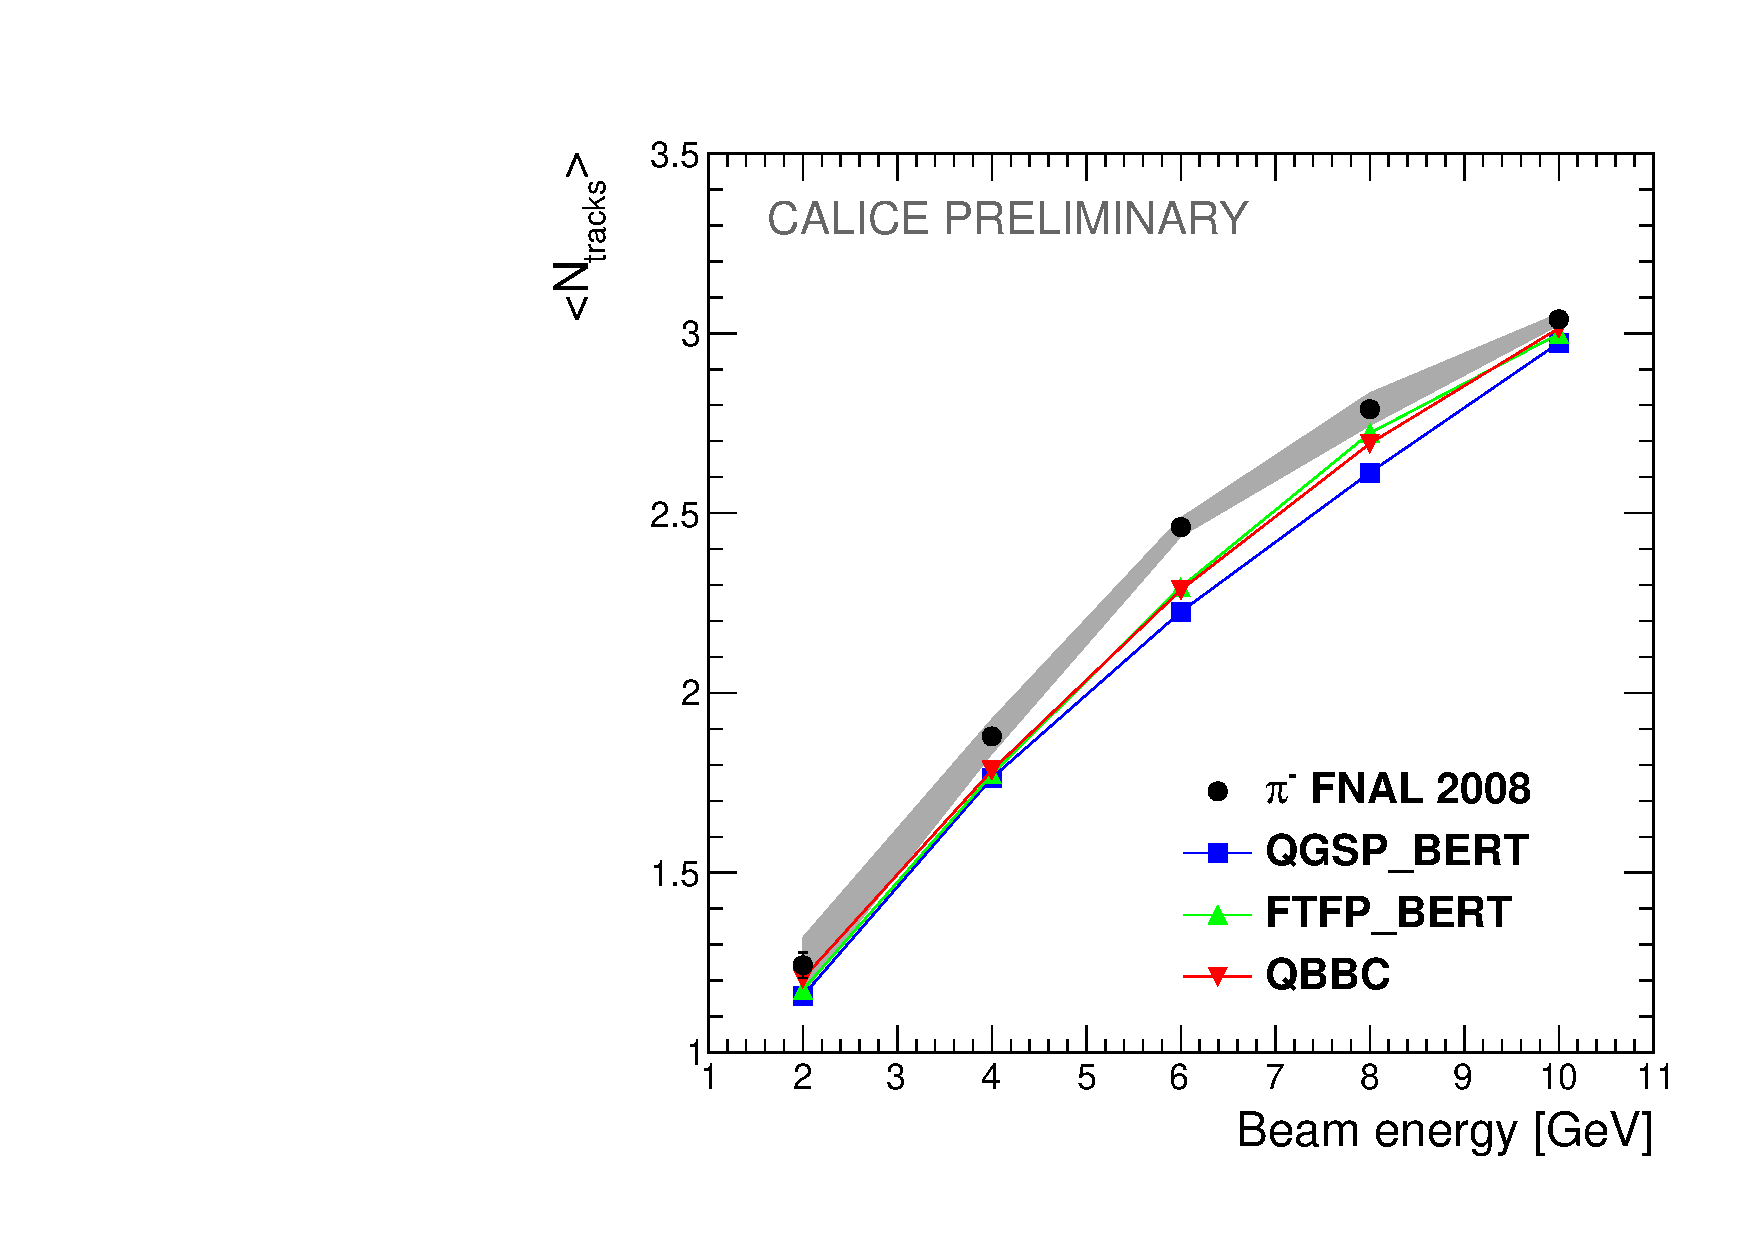
\includegraphics[width=.90\linewidth]{ECAL/plots/ntracks-graph.pdf}
		\caption{\label{fig:tracksgraphF} }
	\end{subfigure}% 
	\begin{subfigure}{0.5\textwidth}
		\centering
		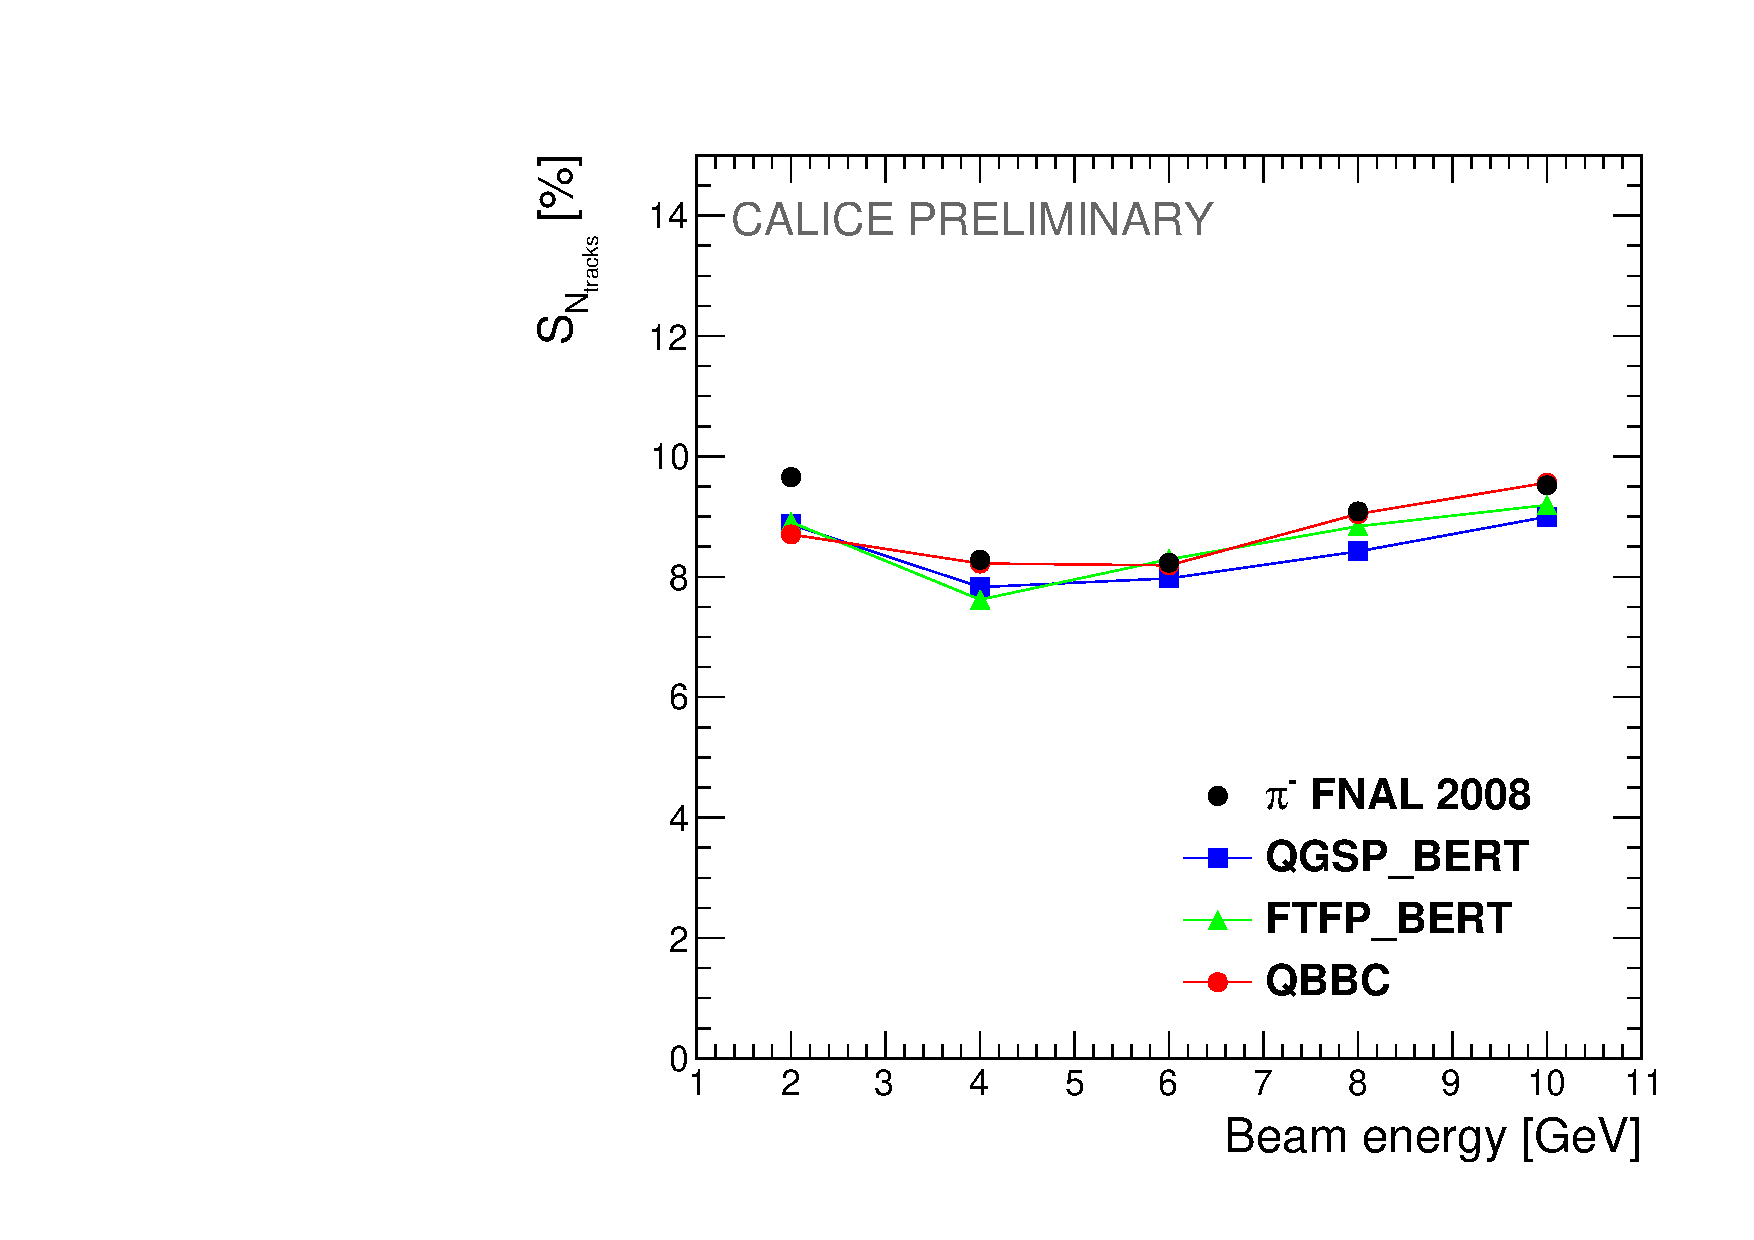
\includegraphics[width=.90\linewidth]{ECAL/plots/ntracks-graph-delta.pdf}
		\caption{\label{fig:dtracksgraphF}}
	\end{subfigure}
	\caption{\label{fig:fulltrackgraphF} \sl Moyenne du nombre des traces trouvées pour les données et les simulations  pour trois listes physiques \geant\ comme une fonction de l'énergie du faisceau (2 \, GeV à 10 \, GeV). }
\end{figure}


%-----------------------------------------------------------------------------
%-----------------------------------------------------------------------------
%-----------------------------------------------------------------------------
\newpage
\subsection*{Les quarks top et bottom \'a l'ILC}

La masse du quark top est comparable à la valeur d'anticipation du vide électrofaible et elle est beaucoup plus élevée que les masses boson du force faible.
\c Ca fait du top quark un sujet de nombreuses théories de la Nouvelle Physique.
Les mesures des propriétés quark bottom, le partenaire du quark top, ont révélé une déviation avec la prédiction de la \sm.
De nombreuses théories \bsm\ prédisent des modifications de la production électro-électrique des paires de quarks lourds par rapport aux attentes de la \sm.
Par conséquent, des mesures précises des couplages de quarks lourds sont nécessaires pour la recherche indirecte de nouvelles particules et la discrimination entre différentes théories.

Cette section se concentre sur la production électrofaible des paires de quarks top et bottom.

La production electrofaible des paires de fermions se déroule à travers le $f\bar{f}X$ vertex, où $X$ représente des bosons vectoriels neutres, un photon ou $Z^0$ boson. Le courant au $f\bar{f}X$ vertex peut être exprimé via les facteurs de forme $F$ comme:
\begin{equation}
\Gamma^{f\bar{f}X}_\mu (k^2,q,\bar{q}) = ie\{ \gamma_\mu (F^X_{1V}(k^2) + \gamma^5 F^X_{1A}(k^2)) - \frac{\sigma_{\mu\nu}(q-\bar{q})^\nu}{2m_f}(iF^X_{2V}(k^2) + \gamma^5 F^X_{2A}(k^2)) \},
\end{equation}
où $k^2= (q+\bar{q})^2$ st le quatri-moment au carré du boson du vecteur échangé, $q$ et $\bar{q} $ sont les quatri-momentes du fermion $f$ et antifermion $\bar{f}$ et $m_f$ est la masse fermion. Les $\gamma_\mu$ et $\gamma_5$ sont les matrices de Dirac, et $\sigma_{\mu\nu} = i/2(\gamma_\mu\gamma_\nu - \gamma_\nu\gamma_\mu)$.

Les valeurs de \sm\ du facteurs de forme sont les suivantes:
\begin{equation}
F^{f\gamma}_{1V} = Q^{f}, \ F^{f\gamma}_{1A} = 0, \ F^{fZ}_{1V} = \frac{I^f - 2Q^f\sin^2\theta_W}{2\cos\theta_W\sin\theta_W}, \ F^{fZ}_{1A} = - \frac{I^f}{2\cos\theta_W\sin\theta_W},
\label{formula:SMformFactors_3F}
\end{equation}
et toutes les facteurs $F_2$ sont zéros. Dans l'equation~\ref{formula:SMformFactors_3F} $I^f$ est  l'isospin faible, $I^t = 1/2$ pour top et $I^b = -1/2$ pour quark bottom  et $Q^f$ est le charge electrique, $Q^t = 2/3$ et $Q^b = -1/3$.

%The form factors are related to fermion couplings with left and right-handed helicity to $Z^0$ boson:
La définition suivante des couplages gauches et droites $Z^0b\bar{b}$ est utilisée tout au long de la thèse: 
\begin{equation}
%g_L^Z = (F_{1V}^Z - F_{1A}^Z), \  g_R^Z = F_{1V}^Z + F_{1A}^Z, 
g_L^Z = I^f - Q^f\sin^2\theta_W, \  g_R^Z = -Q^f\sin^2\theta_W.
\label{formula:EWcouplings_3F}
\end{equation}

L'expression clé pour les études est la section efficace différentielle de $f\bar{f}$ production pour la polarisation du faisceau d'électrons $I=L,R$, exprimée par les facteurs de forme définis:

\begin{multline}
% \frac{\pi\alpha^2 N_c\beta}{s}
\label{formula:DiffSigma_3F}
\frac{d\sigma^I}{d\cos\theta} = \frac{3}{4} \mathcal{A} N_c \beta[ (1+\cos^2\theta) [(\mF_{1V}+\mF_{2V})^2+(\beta \mF_{1A})^2] - \\-4 \cos\theta (\mF_{1V}+\mF_{2V})\beta \mF_{1A} +\\+ \sin^2\theta [\gamma ^{-2} (\mF_{1V} +\gamma^2 \mF_{2V})^2] ]
\end{multline}
où $\mathcal{A} = 4\pi\alpha^2/3s$ avec $\alpha$ comme couplage électromagnétique, $N_c$ est le nombre de couleurs, $\beta$ et $\gamma$ sont la vitesse et le facteur de Lorentz du fermion produit, respectivement.

%-----------------------------------------------------------------------------
%-----------------------------------------------------------------------------
%-----------------------------------------------------------------------------
\newpage
\subsection*{Reconstruction de la charge du quark bottom}
La reconstruction de la section efficace différentielle de quarks lourdes nécessite une mesure de charge précise du quark bottom.
La charge du quark bottom est identifiée en utilisant deux signatures de base:
\begin{itemize}
	\item \textbf{Vertex charge} est une somme de toutes les charges reconstruites, qui sont associées aux sommets de $b$-hadrons.
	\item \textbf{Kaon charge} est une charge de kaons trouvée dans les sommets du hadrons bottom.
\end{itemize}

On a constaté que les algorithmes de vertexing peuvent manquer une ou plusieurs particules des sommets de b-hadron reconstruits. Cet effet diminue la pureté de la charge de vertex.
La procédure de récupération de sommets développée améliore la pureté de la charge de sommets en ajoutant les particules de b-hadron manquantes aux sommets mesurés à l'aide d'un ensemble d'observables reconstruits.

L'identification kaon est possible en utilisant les informations TPC $dE/dx$. Après avoir égalisé le $dE/dx$ dans le spectre angulaire, les kaons des sommets des b-hadrons peuvent être identifiés avec 97\% de pureté et 87\% d'efficacité.

Les graphiques de la pureté de la charge de vertex et le $dE/dx$ en fonction de moment des particules pour hadrons différents sont représentés dans la Fig.~\ref{fig:RecoveryPurityComparison_3F} et la Fig.~\ref{fig:dEdxBefore_3F}, respectivement.

\begin{figure}
	{\centering
		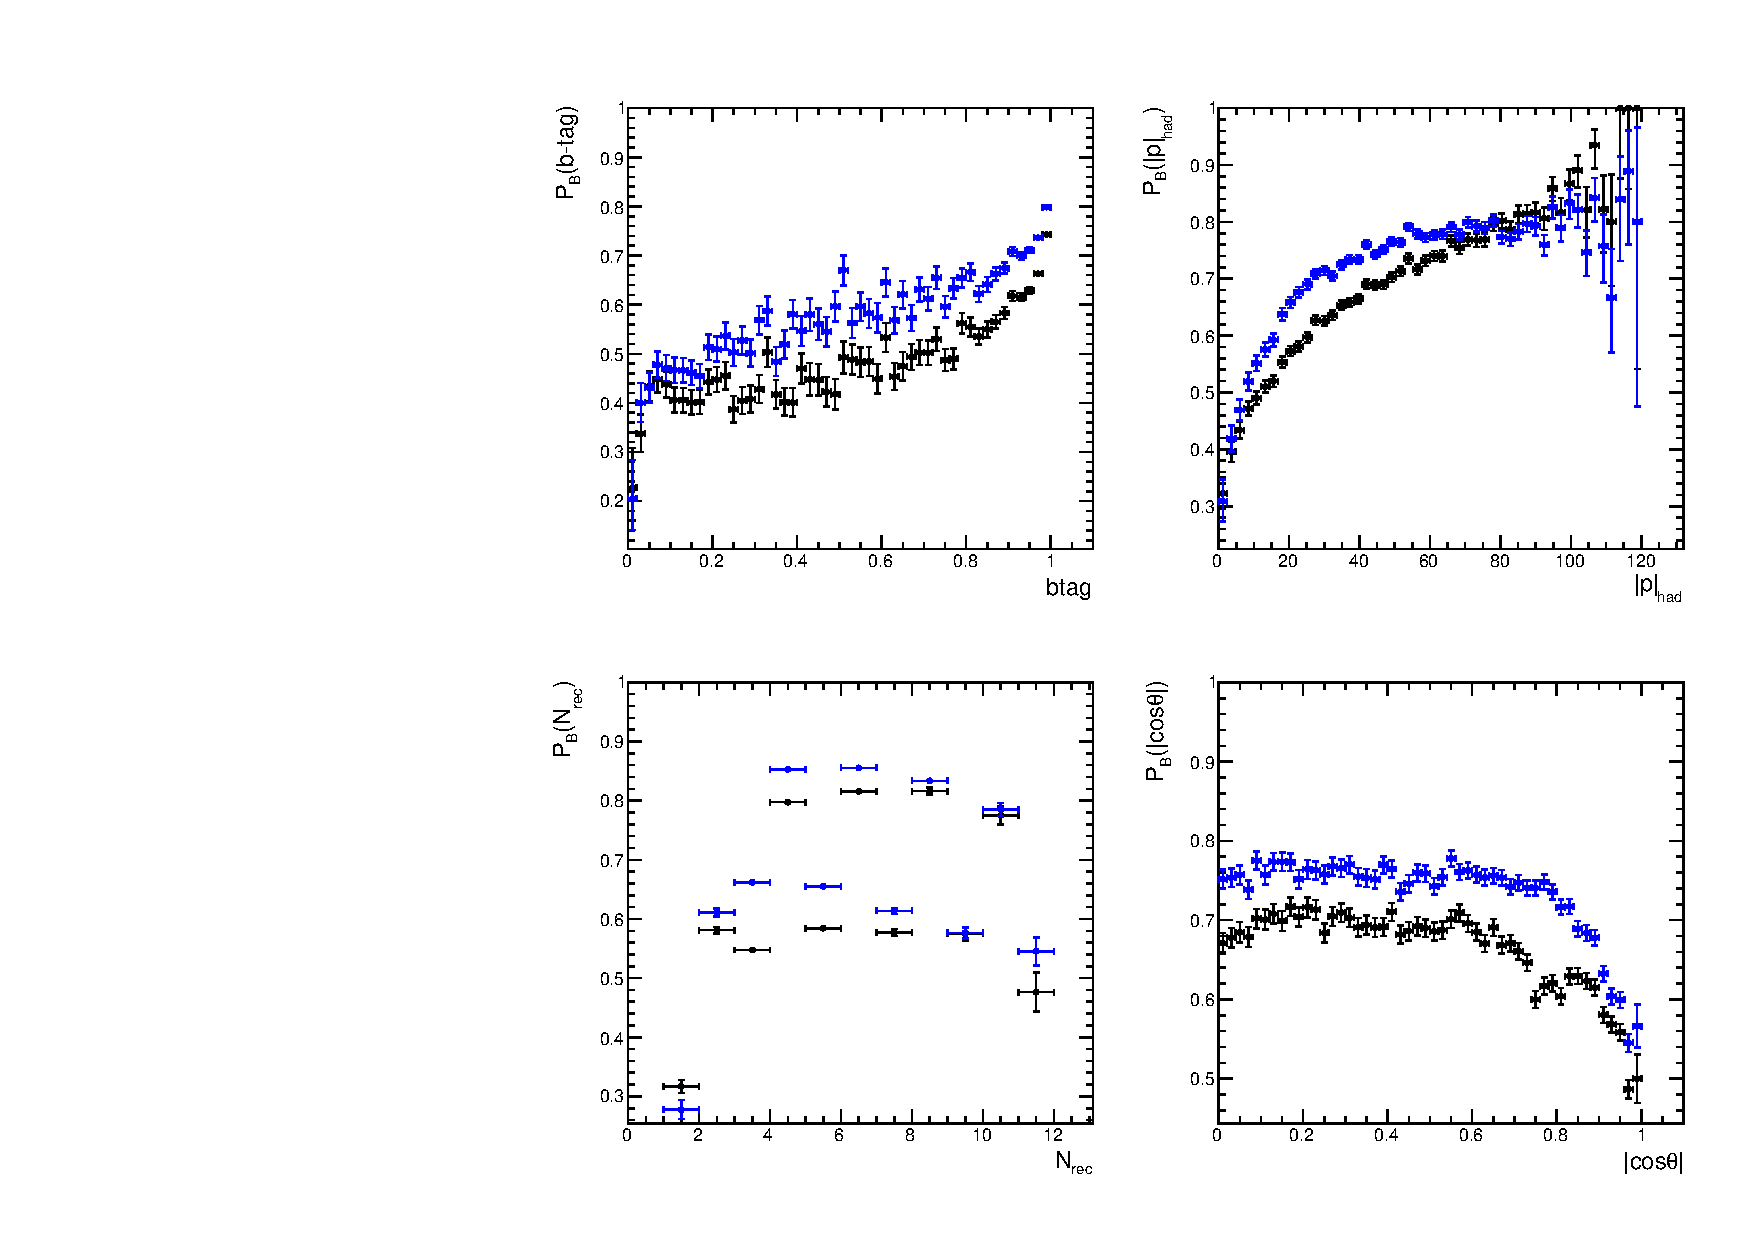
\includegraphics[width=0.95\textwidth]{ILD/plots/recovery-purity-comparison.pdf}
		\caption{\sl Comparaison de la pureté en fonction de b-tag, moment de b-hadron reconstruit, $N_ {rec}$ et l'angle polaire $|\cos\theta|$ avant et après l'algorithme de récupération de vertex. 
		}
		\label{fig:RecoveryPurityComparison_3F}
	}
\end{figure}

\begin{figure}
	{\centering
		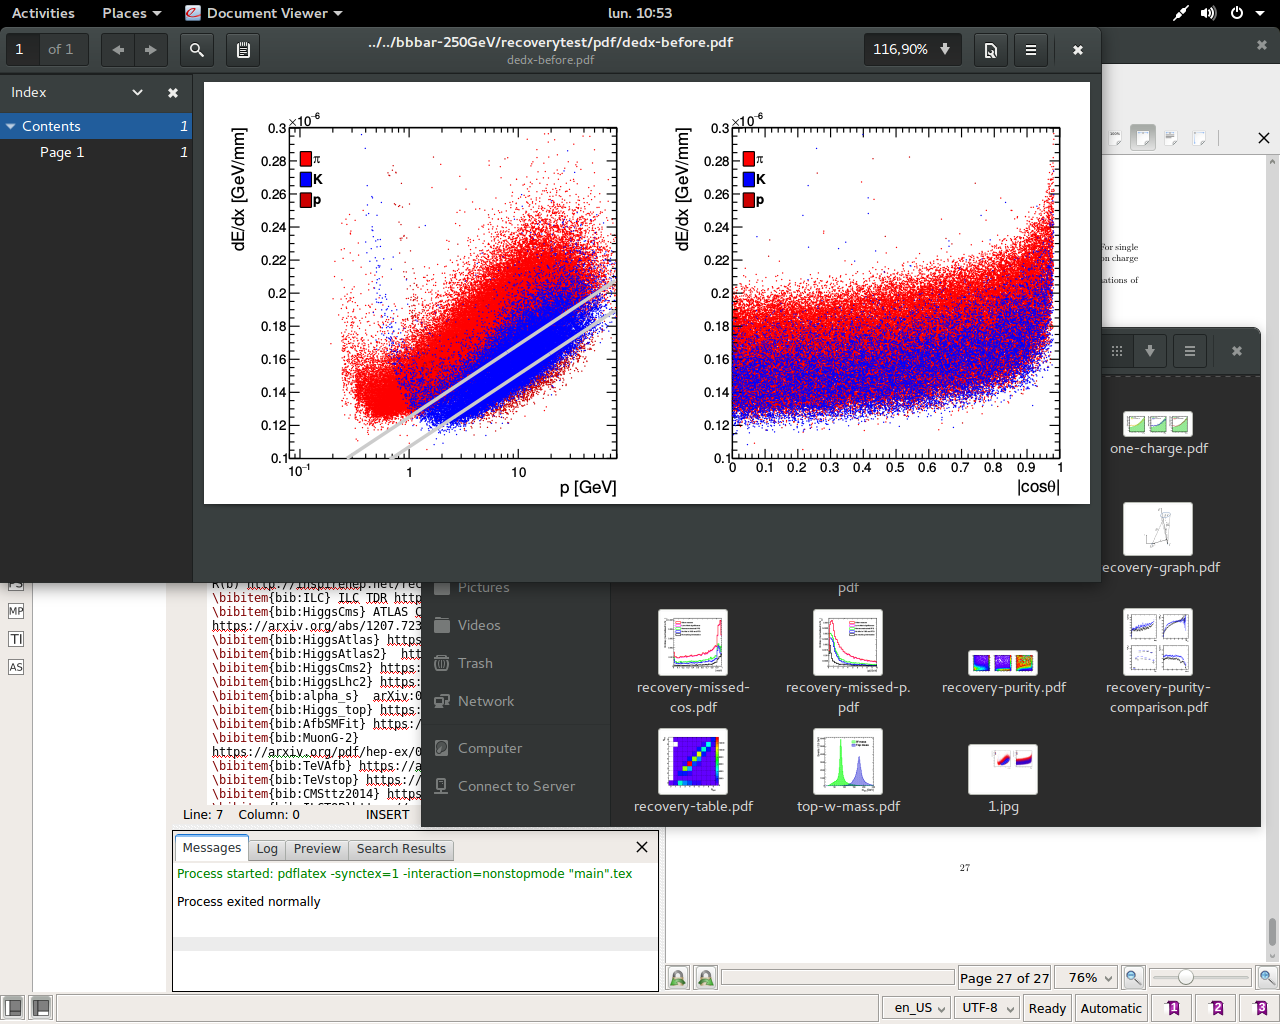
\includegraphics[clip, trim=8cm 18.5cm 7cm 4cm,width=0.95\textwidth]{ILD/plots/dedx-before.png}
		\caption{\sl Le dépôt d'énergie par longueur de trace $dE/dx$ en fonction de moment des particules, l'angle polaire des particules $|\cos\theta|$ pour différentes types des particules. Deux lignes grises séparent la région avec une concentration maximale de kaon.
		}
		\label{fig:dEdxBefore_3F}
	}
\end{figure}

\begin{figure}
	{\centering
		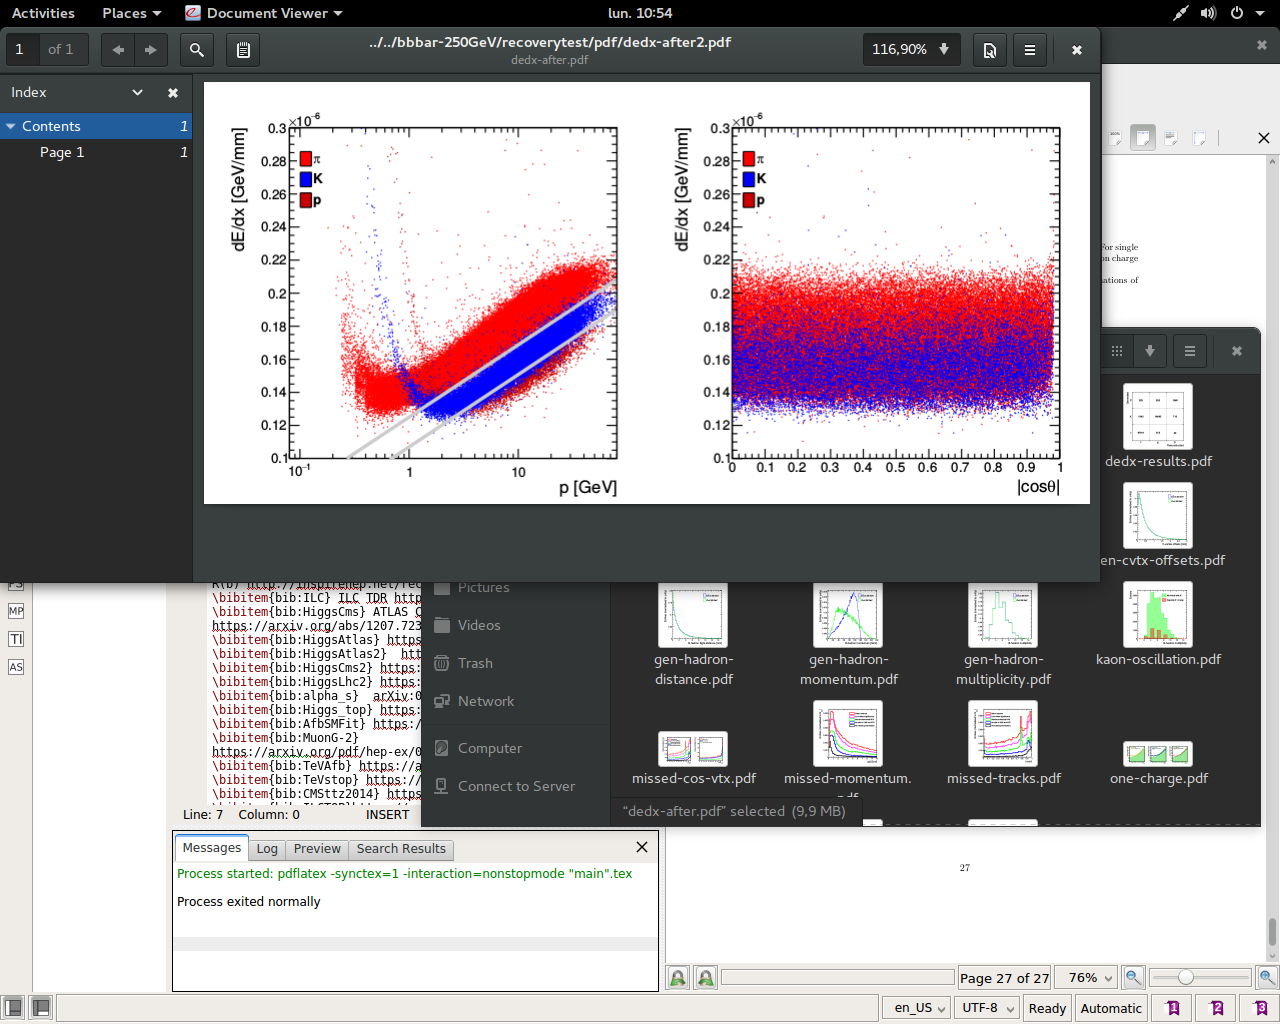
\includegraphics[clip, trim=8cm 18.5cm 7cm 4cm, width=0.95\textwidth]{ILD/plots/dedx-after.png}
		\caption{\sl Le dépôt d'énergie par longueur de trace $dE/dx$ en fonction de moment des particules, l'angle polaire des particules $|\cos\theta|$ pour différentes particules. apr\'es l'application de correction angulaire.  Deux lignes grises séparent la région avec une concentration maximale de kaon.
		}
		\label{fig:dEdxAfter_3F}
	}
\end{figure}


%-----------------------------------------------------------------------------
%-----------------------------------------------------------------------------
%-----------------------------------------------------------------------------
\newpage
\subsection*{Reconstruction de l'angle polaire du quark top et bottom}

L'application de toutes les combinaisons de paires possibles de la charge de sommet, de la charge de kaon et de la charge de $W^\pm$ lepton à la reconstruction de l'angle polaire supérieur illustrée dans la Fig.~\ref {fig:TopAsymmetryChi_3F}.

Cette méthode permet de reconstituer l'asymétrie aussi bon que $A_ {FB}^{rec} / A^{gen}_{FB} = 94\%$ avec l'efficacité finale de 38,6\%, ce qui améliore le résultat précédent~\cite {bib:ILCTOP} par 25\%.

La méthode la plus utilisée est la combinaison de la charge de vertex avec la charge $W^\pm$ lepton car le $ W^\pm$ lepton doit être reconstruit dans chaque événement sélectionné.

\begin{figure}
	\centering
	\begin{subfigure}{0.5\textwidth}
		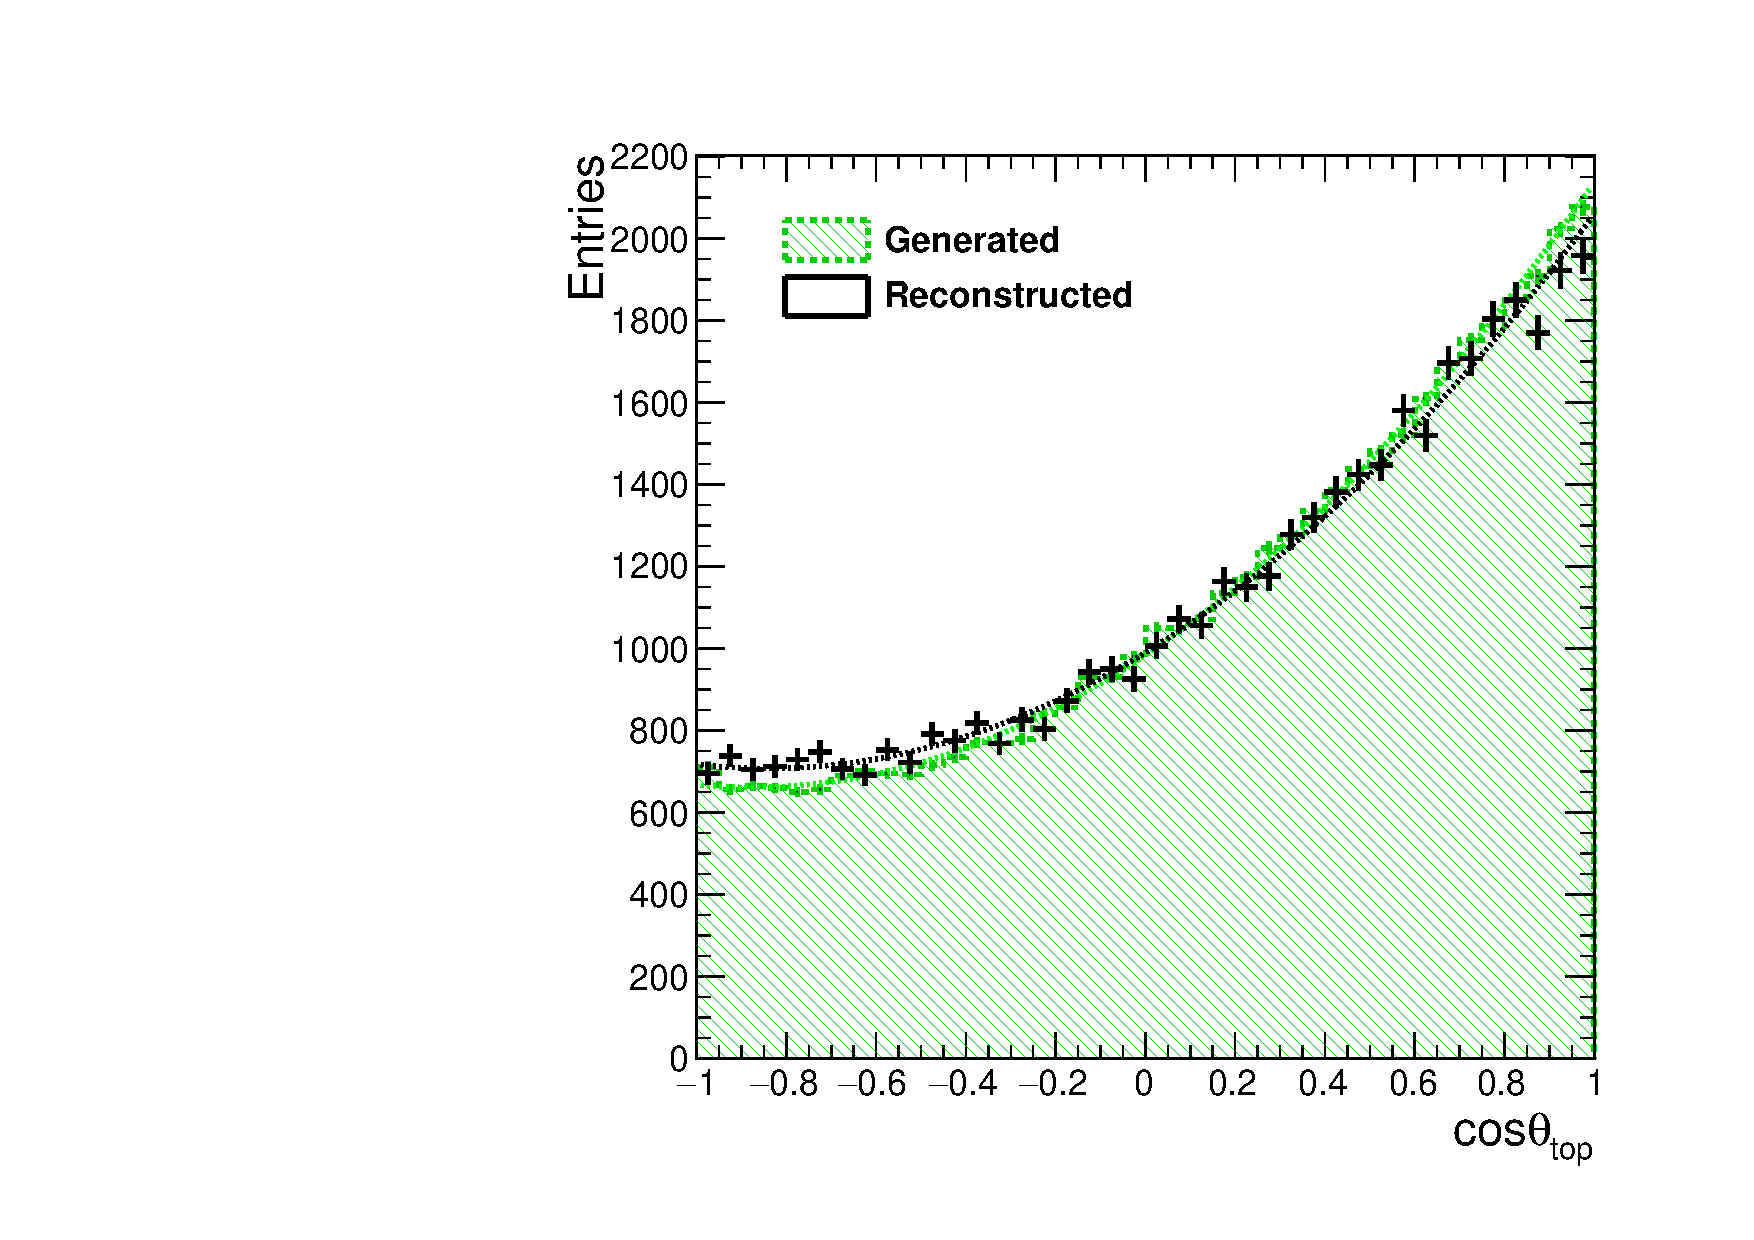
\includegraphics[width=0.95\textwidth]{ILD/plots/top-asymmetry-lepton.pdf}
		\caption{\label{fig:TopAsymmetryChi_a_3F} }
	\end{subfigure}% 
	\begin{subfigure}{0.5\textwidth}
		\centering
		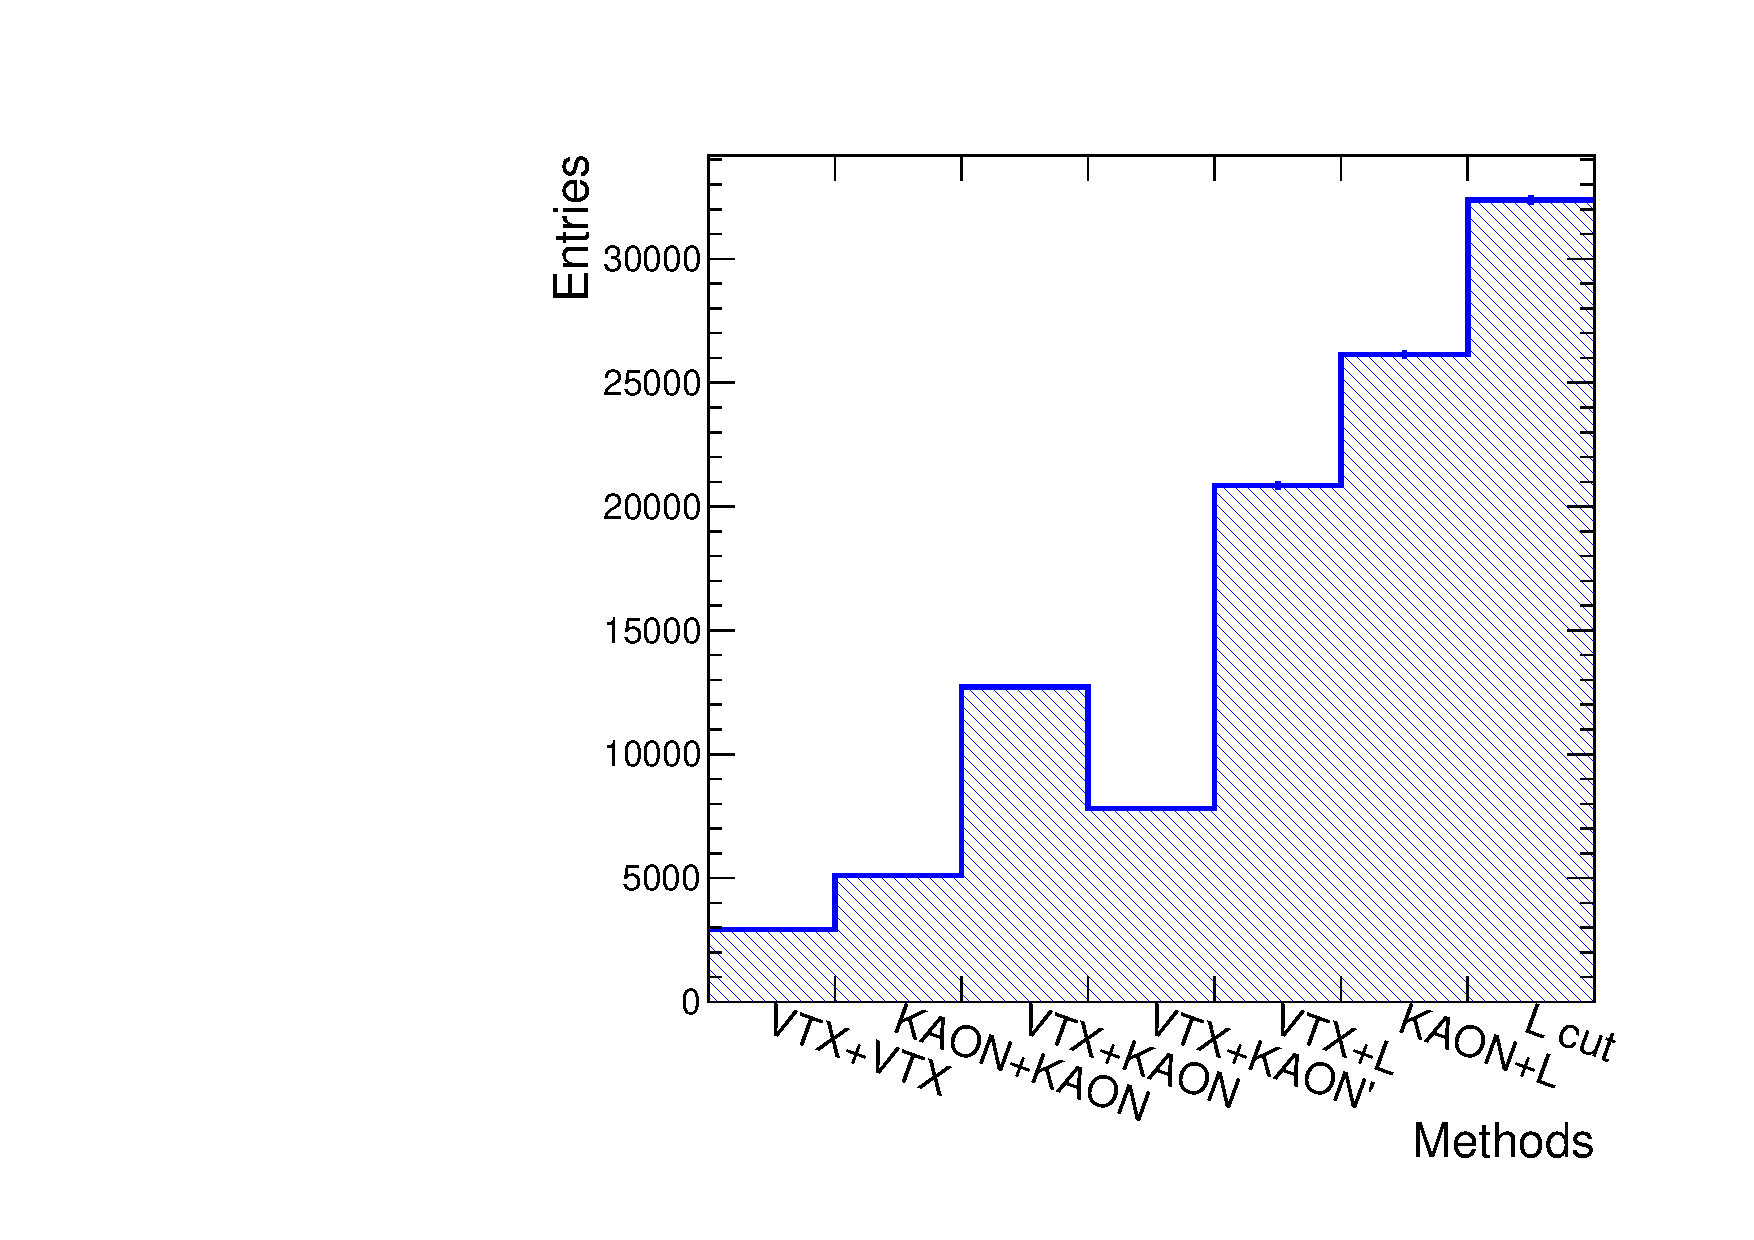
\includegraphics[width=0.95\textwidth]{ILD/plots/top-methods-lepton.pdf}
		\caption{\label{fig:TopAsymmetryChi_b_3F} }
	\end{subfigure}
	\caption{\sl Répartition de l'angle polaire générée par rapport à l'angle polaire reconstruit (a) du quark top en utilisant toutes les combinaisons possibles de signature de charge, tracée en (b).}
	\label{fig:TopAsymmetryChi_3F}
\end{figure}

%-----------------------------------------------------------------------------
%-----------------------------------------------------------------------------
%-----------------------------------------------------------------------------
Les répartitions angulaires polaires reconstruites $b$ à $\sqrt{s} = 250$\,GeV utilisant une combinaison de signatures de charge kaon et vertex sont affich\`ees dans la Fig. ~\ref{fig:BAsymmetryFinal_3F}. La luminosité intégrée $\mathcal{L}_I=250$\,fb$^{-1}$ est supposée pour chaque polarisation du faisceau.

%\subsection*{Reconstruction de l'angle polaire du quark bottom et top}

\begin{figure}
	\centering
	\begin{subfigure}{0.5\textwidth}
		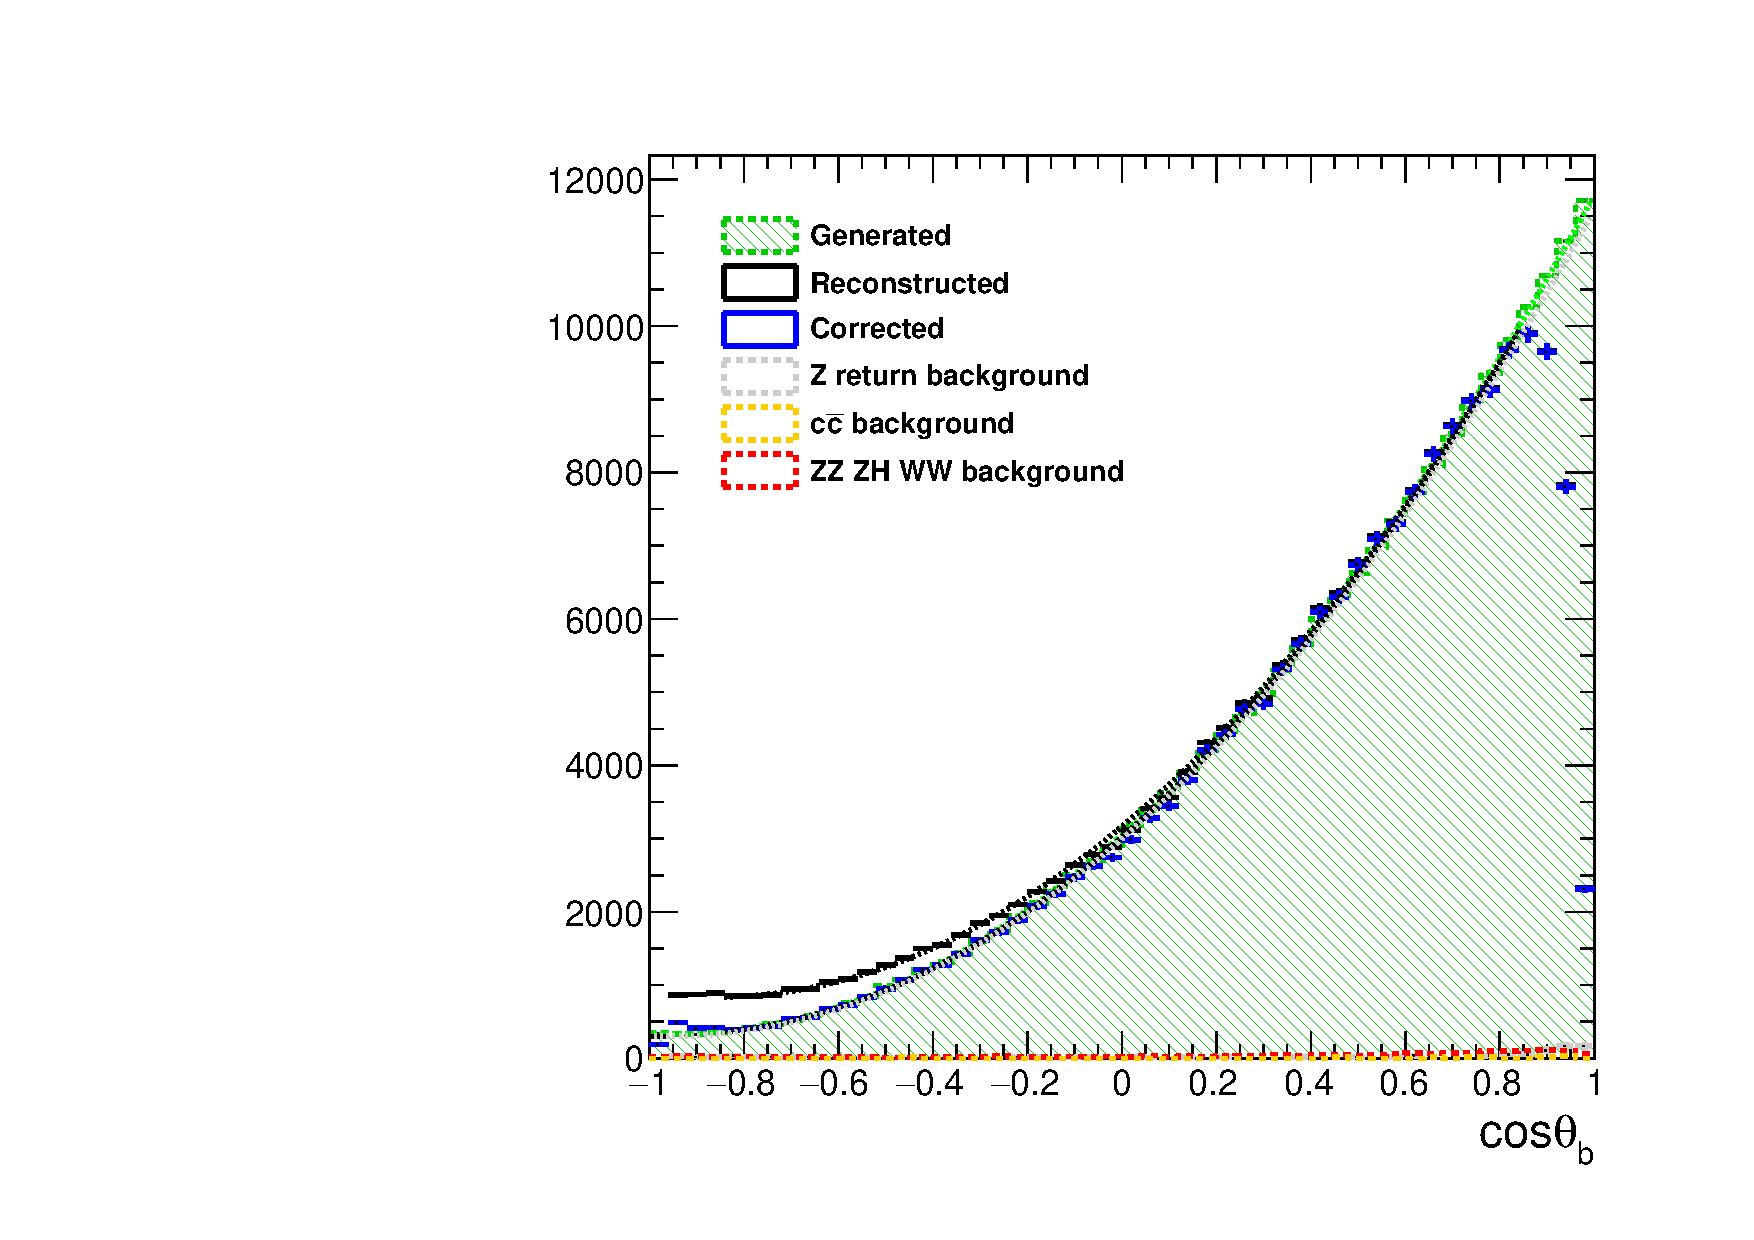
\includegraphics[width=0.95\textwidth]{ILD/plots/basymmetry-final-left.pdf}
		\llap{\shortstack{%
				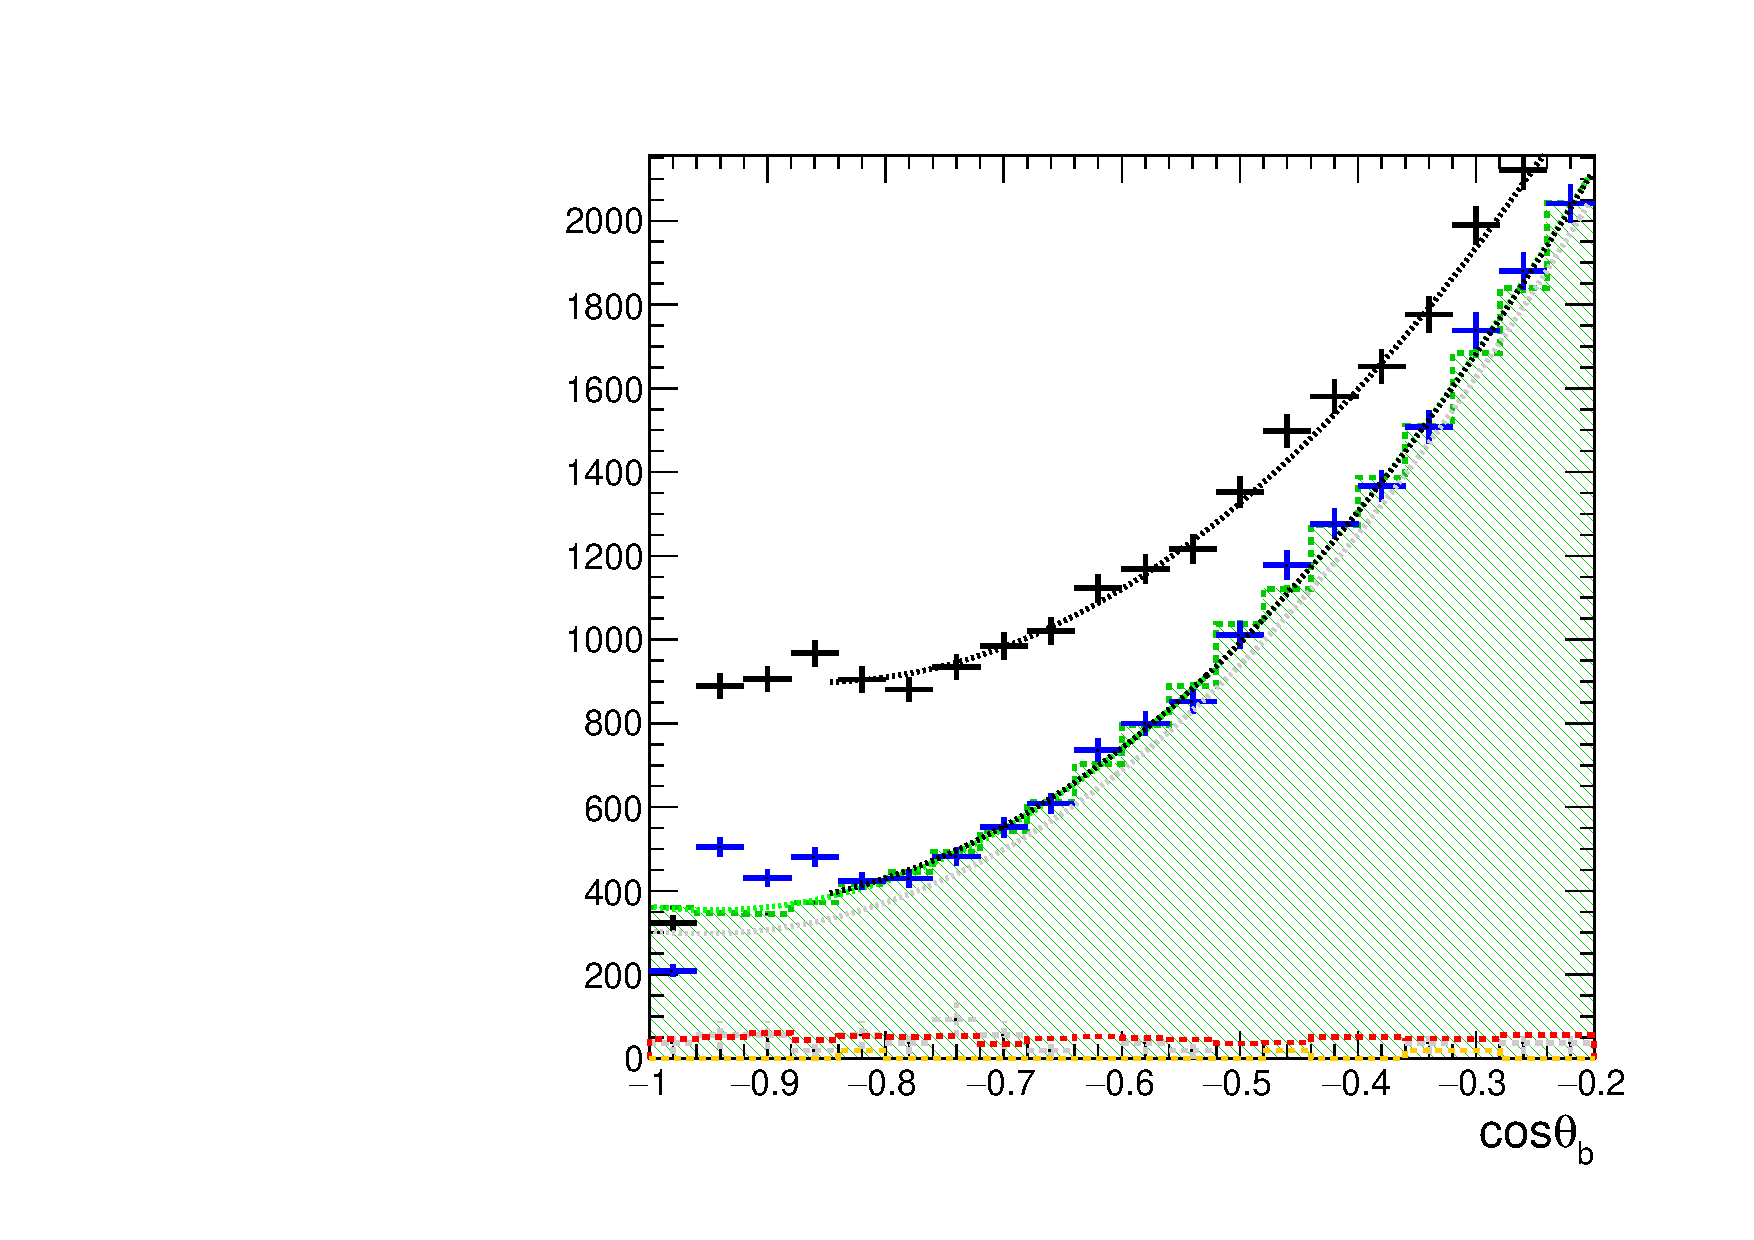
\includegraphics[clip, trim=0cm 0cm 1.8cm 1.7cm, scale=.14]{ILD/plots/zoom-final.pdf}\\
				\rule{0ex}{0.38in}%
			}
			\rule{1.8in}{0ex}}
		\caption{\label{fig:BAsymmetryFinal_a_3F} }
	\end{subfigure}% 
	\begin{subfigure}{0.5\textwidth}
		\centering
		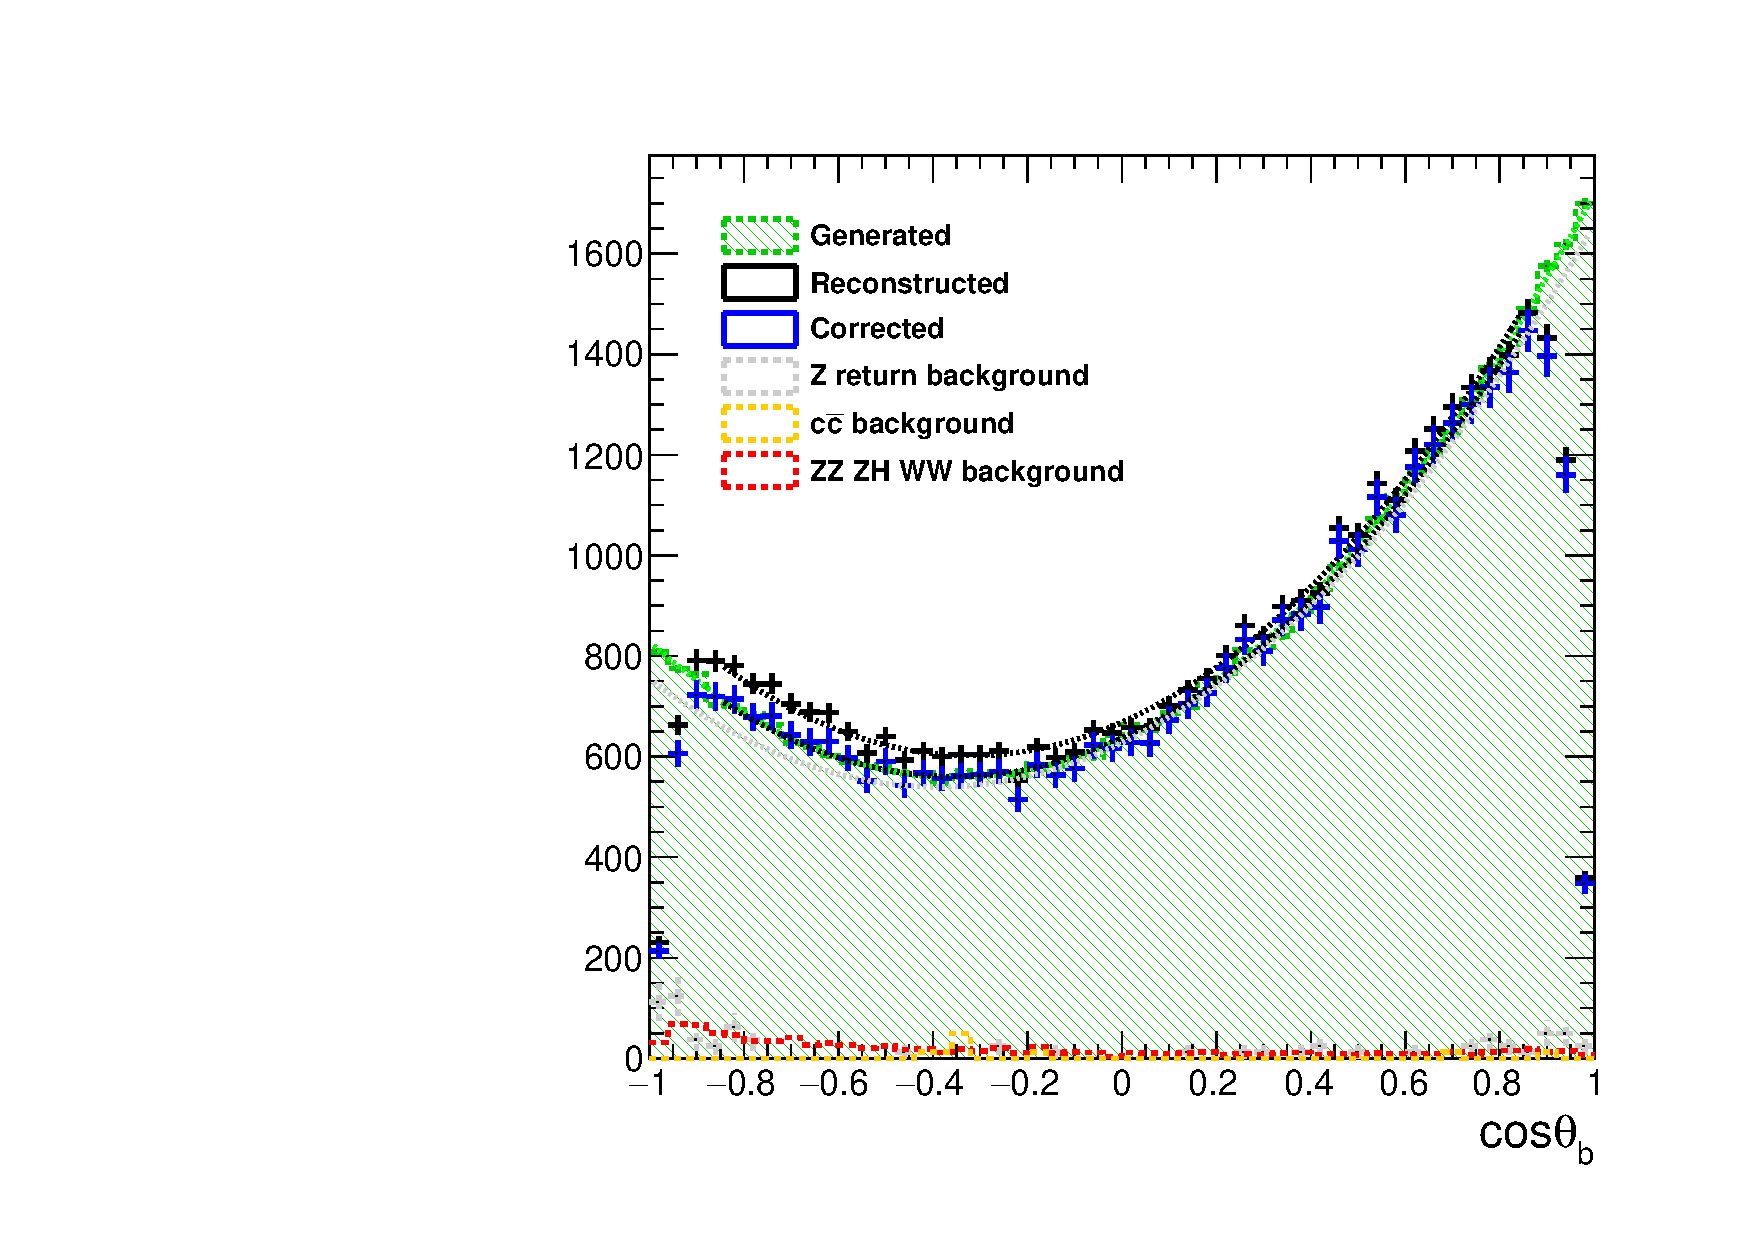
\includegraphics[width=0.95\textwidth]{ILD/plots/basymmetry-final-right.pdf}
		\caption{\label{fig:BAsymmetryFinal_b_3F} }
	\end{subfigure}
	\caption{\sl Distribution d'angle polaire b-quark générée par rapport à l'angle polaire des quarks b reconstruits final dans le cas de gaucher (a) et le cas droitier (b) avec des processus de fond superposés.}
	\label{fig:BAsymmetryFinal_3F}
\end{figure}

La pureté de la charge kaon et vertex est définie à l'aide des événements mesurés avec des charges erronées. En utilisant les puretés mesurées, le spectre reconstruit est corrigé à l'aide d'une procédure basée sur les données.
Les distributions corrigées sont ajustées par une fonction transversale générale, définie comme $S(1+\cos^2\theta) + A\cos\theta$. La précision extraite sur les paramètres $S$ et $A$ est redessinée à la polarisation réaliste $e^-_L, e^+_R = \pm 0.8, \mp 0.3$ et à le partage de luminosité du programme de physique de l'ILC.
Comme on peut le voir à partir de la Fig.~\ref{fig:BAsymmetryFinal_3F}, la contribution des processus de fond de diboson est faible.


Les précisions relatives sur les couplages $Z^0 b\bar{b}$, $g_L^Z$ et $g_R^Z$, pour les mesures LEP~I et pour les performances ILC attendues sont affichées dans la Fig.~\ref{fig:LEPILCResult_3F}.
La précision de l'ILC sur la couplage $g_R^Z$ est suffisante pour confirmer ou rejeter complètement l'influence de New Physics sur les accouplements electroweak $b$ -quark.

\begin{figure}
	\centering
	\begin{subfigure}{0.5\textwidth}
		\includegraphics[width=0.99\textwidth]{ILD/plots/lep-result-zoom.pdf}
		\caption{\label{fig:LEPILCResult_a_3F} }
	\end{subfigure}% 
	\begin{subfigure}{0.5\textwidth}
		\centering
		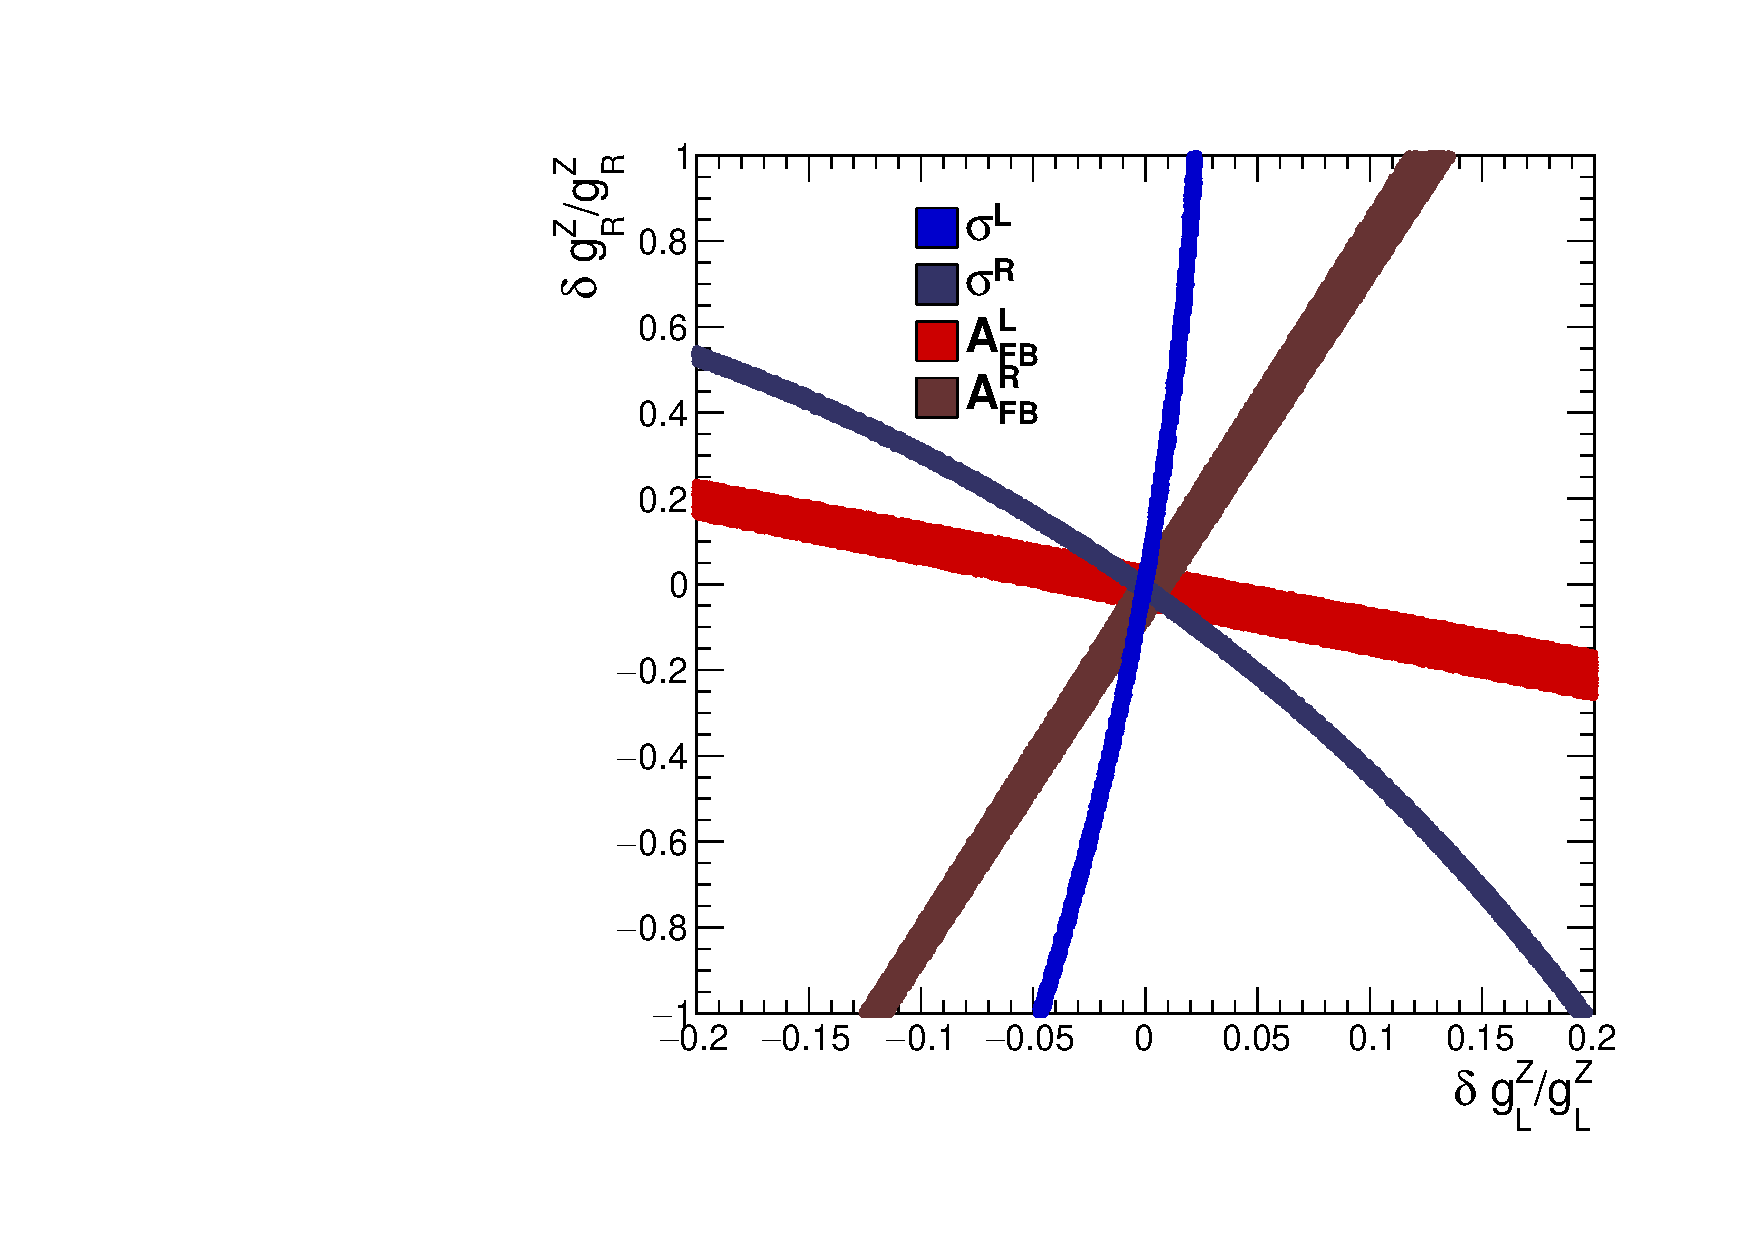
\includegraphics[width=0.99\textwidth]{ILD/plots/ilc-result.pdf}
		\caption{\label{fig:LEPILCResult_b_3F} }
	\end{subfigure}
	\caption{\sl Les régions de $\pm 1\,\sigma$ sur les couplages $Z^0b\bar{b}$ définies par l'asymétrie avant-arrière et les mesures transversales totales au LEP (a) et ILC via l'ajustement de la section transversale différentielle (b). Les lignes directrices détaillées montrent la valeur \sm. La région autorisée attendue à l'ILC est centrée sur les valeurs de couplage de \sm.}
	\label{fig:LEPILCResult_3F}
\end{figure}

\subsection*{Conclusions}

Cette thèse présente de nouvelles méthodes et études développées pour le projet de l'ILC.
Les détecteurs de l'ILC sont conçus pour l'application d'algorithmes de flux de particules, qui améliorent les performances physiques en utilisant les informations des calorimètres hautement granulaires.

Le prototype de calorim\`etre \'electromagn\'etique hautement granulaire a été construit et testé par la collaboration CALICE.
Au cours de cette thèse, un algorithme de recherche de traces a été développé permettant de reconstruire des traces secondaires issues des interactions hadroniques dans le prototype SiW-ECAL.
La simulation de SiW-ECAL a été comparée aux données en utilisant les nouvelles observables de l'algorithme de recherche de traces.

Tous les modèles de simulation testés montrent une bonne performance en termes de nouveaux observables.

Dans cette thèse, la technique de charge du quark bottom est utilisée pour la reconstruction de la distribution de l'angle polaire du quark top et bottom.
Les méthodes développées sont appliquées dans deux canaux $e^+ e^- \to t\bar{t}$ et $e^+ e^- \to b\bar{b}$ processes à $\sqrt {s} = 500$\,GeV et 250\,GeV, respectivement.

La procédure de mesure de la pureté de charge par les données permet de corriger la distribution  de l'angle polaire pour la contamination résiduelle.
En conséquence, l'angle polaire du quark bottom reconstruit est utilisable pour l'extraction des couplages  et des facteurs de forme électrofaibles du quark bottom.
La précision prévue à l'ILC sur le couplage droite $Zb\bar{b}$ est 5 fois meilleur qu'au LEP, l'anomalie LEP sera soit totalement confirmée, ou soit définitivement écartée.


